\documentclass[12pt]{article}
\usepackage[margin=2.5cm]{geometry}
\usepackage{enumerate}
\usepackage{amsfonts}
\usepackage{amsmath}
\usepackage{fancyhdr}
\usepackage{amsmath}
\usepackage{amssymb}
\usepackage{amsthm}
\usepackage{mdframed}
\usepackage{graphicx}
\usepackage{subcaption}
\usepackage{listings}
\usepackage{xcolor}
\usepackage[utf]{kotex}


\begin{document}
\title{Problem Set 4 Solution}
\author{Hyungmo Gu}
\maketitle

\section*{Question 1}
\begin{enumerate}[a.]
    \item

    \textbf{Statement:} $\forall f,g:\mathbb{N} \to \mathbb{R}^{+}$,
    $b \in \mathbb{R}^{+}$, $(g(n) \in \Theta(f(n))) \land (n_0 \in \mathbb{N},\:
    n \geq n_0 \Rightarrow f(n) \geq b \land g(n) \geq b) \land (b > 1) \Rightarrow
    \log_b(g(n)) \in \Theta(\log_b(f(n)))$

    \bigskip

    \textbf{Statement Expanded:} $\forall f,g:\mathbb{N} \to \mathbb{R}^{+}$,
    $b \in \mathbb{R}^{+}$, $\Bigl(\exists c_1,c_2,n_0 \in \mathbb{R}^{+},\:\forall n \in \mathbb{N},\:
    n \geq n_0 \Rightarrow c_1 \cdot g(n) \leq f(n) \leq c_2 \cdot g(n)\Bigr) \land \Bigl(\exists n_1 \in \mathbb{N},\:
    n \geq n_1 \Rightarrow f(n) \geq b \land g(n) \geq b \Bigr) \land \Bigl( b > 1 \Bigr) \Rightarrow
    \Bigl(\exists d_1,d_2,n_2 \in \mathbb{R}^{+},\:\forall n \in \mathbb{N},\: n \geq n_2
    \Rightarrow d_1 \cdot \log_b(g(n)) \leq \log_b(f(n)) \leq d_2 \cdot \log_b(g(n) \Bigr)$

    \bigskip

    \begin{proof}
        Let $f,g:\mathbb{N} \to \mathbb{R}^{+}$, and $b \in \mathbb{R}^{+}$. Assume
        $c_1 = 1$, $c_2 = b$, and $n_0 = 1$, and $n \in \mathbb{N}$ such that
        $n \geq n_0$ and $c_1 \cdot g(n) \leq f(n) \leq c_2 \cdot g(n)$. Assume $f(n)$
        and $g(n)$ are eventually $\geq b$. Assume $b > 1$. Let $d_1 = 1$, $d_2 = 2$,
        and $n_2 = n_0$. Assume $n \geq n_2$.

        \bigskip

        We need to show $d_1 \cdot \log_b g(n) \leq \log_b f(n) \leq d_2 \cdot \log_b g(n)$.

        \bigskip

        We will do so in two parts. One for $(d_1 \cdot \log_b g(n) \leq \log_b f(n))$ and
        the other for $(\log_b f(n) \leq d_2 \cdot \log_b g(n))$.

        \bigskip

        \textbf{Part 1 ($d_1 \cdot \log_b g(n) \leq \log_b f(n)$):}

        \bigskip

        The assumption tell us

        \begin{align}
            c_1 \cdot g(n) \leq f(n)
        \end{align}

        \bigskip

        Then, it follows from the fact $\forall x,y \in \mathbb{R}^{+}, x \geq y
        \Leftrightarrow \log x \geq \log y$

        \begin{align}
            \log (c_1 \cdot g(n)) &\leq \log (f(n))
        \end{align}

        \bigskip

        Then, using the fact $b > 1$, we can calculate

        \begin{align}
            \frac{\log (c_1 \cdot g(n))}{\log b} &\leq \frac{\log (f(n))}{\log b}\\
            \frac{\log (c_1) + \log (g(n))}{\log b} &\leq \frac{\log (f(n))}{\log b}
        \end{align}

        \bigskip

        Then,

        \begin{align}
            \frac{\log (g(n))}{\log b} &\leq \frac{\log (f(n))}{\log b}
        \end{align}

        by the fact $c_1 = 1$ and $\log c_1 = 0$.

        \bigskip

        Then, since $\frac{\log f(x)}{\log b} = \log_b f(x)$,

        \begin{align}
            \log_b (g(n)) &\leq \log_b (f(n))
        \end{align}

        \bigskip

        Then, because we know $d_1 = 1$, we can conclude

        \begin{align}
            \log_b (g(n)) &\leq d_1 \cdot \log_b (f(n))
        \end{align}


        \bigskip

        \textbf{Part 2 ($\log_b f(n) \leq d_2 \cdot \log_b g(n)$):}

        \bigskip

        The assumption tells us

        \begin{align}
            f(n) &\leq c_2 \cdot g(n)
        \end{align}

        \bigskip

        Then, it follows from the fact $\forall x,y \in \mathbb{R}^{+}, x \geq y
        \Leftrightarrow \log x \geq \log y$

        \begin{align}
            \log (f(n)) &\leq \log (c_2 \cdot g(n))
        \end{align}

        \bigskip

        Then, using the fact $b > 1$, we can calculate

        \begin{align}
            \frac{\log (f(n))}{\log b} &\leq \frac{\log (c_2 \cdot g(n))}{\log b}\\
            \frac{\log (f(n))}{\log b} &\leq \frac{\log (c_2) + \log (g(n))}{\log b}
        \end{align}

        \bigskip

        Then, since $c_2 = b$,

        \begin{align}
            \frac{\log (f(n))}{\log b} &\leq \frac{\log (b) + \log (g(n))}{\log b}
        \end{align}

        \bigskip

        Then, using the fact $g(n)$ is eventually $\geq b$, we can write

        \begin{align}
            \frac{\log (f(n))}{\log b} &\leq \frac{\log (g(n)) + \log (g(n))}{\log b}\\
            \frac{\log (f(n))}{\log b} &\leq \frac{2 \cdot \log (g(n))}{\log b}
        \end{align}

        \bigskip

        Then, since $\frac{\log f(x)}{\log b} = \log_b f(x)$,

        \begin{align}
            \log_b (f(n)) &\leq 2 \cdot \log_b (g(n))
        \end{align}

        \bigskip

        Then, because we know $d_2 = 2$, we can conclude

        \begin{align}
            \log_b (f(n)) &\leq d_2 \cdot \log_b (g(n))
        \end{align}
    \end{proof}

    \textbf{Notes:}

    \begin{itemize}
        \item $\forall x,y \in \mathbb{R}^{+}, x \geq y \Leftrightarrow \log x \geq \log y$


        \item $\exists c_1,c_2,n_0 \in \mathbb{R}^{+},\:\forall n \in \mathbb{N},
        n \geq n_0 \Rightarrow c_1 \cdot g(n) \leq f(n) \leq c2 \cdot g(n)$

        \item \textbf{Definition of Eventually:} $\exists n_0 \in \mathbb{N},
        n \geq n_0 \Rightarrow P$, where $P:\mathbb{N} \to \{\text{True},\text{False}\}$
    \end{itemize}

    \item

    \begin{proof}
        Let $k \in \mathbb{N}$.

        \bigskip

        First, we will analyze the cost of loop 2 over iteration of loop 1.

        \bigskip

        The code tells us loop 2 starts at $j_k = 1$ with $j_k$ increasing by
        a factor of 3 per iteration until $j_k \geq 1$.

        \bigskip

        Using these facts, we can calculate that the terminating condition occurs
        when

        \setcounter{equation}{0}
        \begin{align}
            3^k &\geq i\\
            k &\geq \log_3 i
        \end{align}

        \bigskip

        Because we know the number of iterations is the smallest value of $k$
        satisfying the above inequality, we can conclude loop 2 has

        \begin{align}
            \lceil \log_3 i \rceil
        \end{align}

        iterations.

        \bigskip

        Next, we need to determine the total number of iterations of loop 2
        over all iterations of loop 1.

        \bigskip

        The code tells us loop 1 starts at $i = 1$ and ends at $i = n$ with each
        $i$ increasing by 1 per iteration.

        \bigskip

        Using these facts, we can conclude loop 2 has total of

        \begin{align}
            \lceil \log_3 1 \rceil + \lceil \log_3 2 \rceil + \cdots + \lceil \log_3 n \rceil &= \sum\limits_{i=1}^n \lceil \log_3 i \rceil
        \end{align}

        iterations.
    \end{proof}

    \item
    After scratching head and looking at solution many times, I realized that there
    are many things I do not yet understand, and it's the best to write what I have
    and learn from the solution. Here is my best attempt :).

    \begin{proof}
        Let $n \in \mathbb{N}$.

        \bigskip

        The previous answer tells us the exact cost of the algorithm is
        \setcounter{equation}{0}
        \begin{align}
            \sum\limits_{i=1}^n \lceil \log_3 i \rceil
        \end{align}

        Then, it follows by changing the variable $i$ to $i' = \log_3 i$ we can write

        \begin{align}
            \sum\limits_{i'=0}^{\lceil \log_3 n \rceil} i'
        \end{align}

        \bigskip

        Then, because we know $\sum\limits_{i=0}^n i = \frac{n(n+1)}{2}$, we can
        conclude

        \begin{align}
            \sum\limits_{i'=0}^{\lceil \log_3 n \rceil} i' &= \frac{(\lceil \log_3 n \rceil)(\lceil \log_3 n \rceil + 1)}{2}\\
            &= \frac{\lceil \log_3 n \rceil^2 + \lceil \log_3 n\rceil}{2}
        \end{align}

        \bigskip

        Then, we can conclude the runtime of the algorithm is $\Theta(\log_3^2 n)$.
    \end{proof}

    \bigskip

    \begin{mdframed}
        \underline{\textbf{Correct Solution:}}

        \bigskip

        \color{red}
        We need to determne $\Theta$ of the algorithm.

        \bigskip

        We will prove that the $\Theta$ of the algorithm is $\Theta(n\log n)$.

        \bigskip

        The answer to previous question tells us the total exact cost of the
        algorithm is

        \begin{align}
            \sum\limits_{i=1}^n \lceil \log_3 i \rceil
        \end{align}

        \bigskip

        Then, by using fact 1 $\forall x \in \mathbb{R}, x \leq \lceil x \rceil \leq x + 1$,
        we can calculate

        \begin{align}
            \sum\limits_{i=1}^n \log_3 i &\leq \sum\limits_{i=1}^n \lceil \log_3 i \rceil \leq \sum\limits_{i=1}^n \Bigl( \log_3 i + 1 \Bigr)\\
            \sum\limits_{i=1}^n \log_3 i &\leq \sum\limits_{i=1}^n \lceil \log_3 i \rceil \leq \Bigl(\sum\limits_{i=1}^n \log_3 i + \sum\limits_{i=1}^n 1 \Bigr)\\
            \sum\limits_{i=1}^n \log_3 i &\leq \sum\limits_{i=1}^n \lceil \log_3 i \rceil \leq \sum\limits_{i=1}^n \log_3 i + n
        \end{align}

        \bigskip

        Then,

        \begin{align}
            \log_3 \Bigl(\prod\limits_{i=1}^n i \Bigr) &\leq \sum\limits_{i=1}^n \lceil \log_3 i \rceil \leq \log_3 \Bigl(\prod\limits_{i=1}^n i \Bigr) + n\\
            \log_3 (n!) &\leq \sum\limits_{i=1}^n \lceil \log_3 i \rceil \leq \log_3 (n!) + n
        \end{align}

        by the fact $\forall a,b \in \mathbb{R}^{+}, \log (a) + \log (b) = \log (ab)$.

        \bigskip

        Then,

        \begin{align}
            \frac{\ln n!}{\ln 3} &\leq \sum\limits_{i=1}^n \lceil \log_3 i \rceil \leq \frac{\ln (n!)}{\ln 3} + n
        \end{align}

        by changing the base to $e$ using the formula $\log_3 n! = \frac{\log_e n!}{\log_e 3} = \frac{\ln n!}{\ln 3}$.

        \bigskip

        Now, the fact 2 tells us $n! \in \Theta (e^{n\ln n - n + \frac{1}{2}\ln n})$.

        \bigskip

        Because we know from fact 3 that $n\ln n - n + \frac{1}{2}\ln n$ is
        eventually $\geq 1$, we can conclude $e^{n\ln n - n \frac{1}{2} \ln n}$ is
        eventually $\geq e$.

        \bigskip

        Since $n!$ is also eventually $\geq e$, by using solution to problem 1.a with
        $g(n) = n!$ and $f(n) = e^{n\ln n - n + \frac{1}{2}\ln }$ and $b = e$,
        we can write

        \begin{align}
            \ln(n!) \in \Theta(\ln(e^{n\ln n - n + \frac{1}{2}\ln n}))\\
            \ln(n!) \in \Theta(n\ln n - n + \frac{1}{2}\ln n)
        \end{align}

        \bigskip

        Then,

        \begin{align}
            \ln(n!) \in \Theta(n\ln n)
        \end{align}

        by the fact $n \ln n - n + \frac{1}{2} \ln n \in \Theta(n \ln n)$.

        \bigskip

        So, since the algorithm runs at least $\frac{\ln n!}{\ln 3}$, we can
        conclude it has asymptotic lower bound of $\Omega(n \ln n)$, and since
        the algorithm runs at most $\frac{\ln n!}{\ln 3} + n$, we can conclude it
        has upper bound running time of $\mathcal{O}(n\ln n)$.

        \bigskip

        Since the value of $\Omega$ and $\mathcal{O}$ are the same, we can conclude
        the algorithm has running time of $\Theta(n \ln n)$ or $\Theta(n \log n)$.
        \color{black}

    \end{mdframed}

    \bigskip

    \textbf{Notes:}

    \begin{itemize}
        \item In a main flow of proof, when there is a huge interruption like
        showing $\ln(n!) \in \Theta(n\ln n)$, how can a sentence be started to tell
        the audience we are working on another major idea?

        \item When an interruption in proof has been occured for another
        major part of a proof, how can a sentence be started to combine
        parts together?

        \item How can a sentence be written to say condition $x_1$, $x_2$, and $x_3$
        are satisfied, so a statement $y$ can be used to an equation or an idea?

    \end{itemize}
\end{enumerate}

\section*{Question 2}
\begin{enumerate}[a.]
    \item

    We need to evaluate tight asymptotic upper bound.

    \bigskip

    We will prove that the tight asymptotic upper bound of the algorithm is
    $\mathcal{O}(n^2)$.

    \bigskip

    First, we need to analyze the number of iterations of loop 2 per iteration of
    loop 1.

    \bigskip

    The code tells us loop 2 starts at $j = 0$ and ends at most$j = i - 1$ with
    $j$ increasing by 1 per iteration.

    \bigskip

    Then, using these facts, we can conclude loop 2 has at most

    \setcounter{equation}{0}
    \begin{align}
        \left\lceil \frac{i-1-0+1}{1} \right\rceil = i
    \end{align}

    iterations.

    \bigskip

    Next, we need to determine the total number of iterations of loop 2 over all
    iterations of loop 1.

    \bigskip

    The code tells us that loop 1 starts at $i = n$ and ends at most $i = 0$ with
    $i$ decreasing by 1 per iteration.

    \bigskip

    Because we know each iteration of loop 1 takes $i$ iterations by loop 2, using
    these facts, we can conclude the total number of iterations of loop 2 is at most

    \begin{align}
        n + (n-1) + (n-2) + \cdots + 0 &= \sum\limits_{i=1}^n\\
        &= \frac{n(n+1)}{2}
    \end{align}

    iterations, or $\mathcal{O}(n^2)$.

    \bigskip

    \begin{mdframed}
        \underline{\textbf{Correct Solution:}}

        \bigskip

        We need to evaluate tight asymptotic upper bound.

        \bigskip

        We will prove that the tight asymptotic upper bound of the algorithm is
        $\mathcal{O}(n^2)$.

        \bigskip

        \color{red}First, we need to analyze the cost of loop 2.\color{black}

        \bigskip

        The code tells us loop 2 starts at $j = 0$ and ends at most$j = i - 1$ with
        $j$ increasing by 1 per iteration.

        \bigskip

        \color{red}
        Then, since each iteration of loop 2 takes a constant step (1 step), using these facts,
        we can conclude the cost of loop 2 is at most

        \setcounter{equation}{0}
        \begin{align}
            1 \cdot (i-1-0+ 1) = i
        \end{align}

        steps.
        \color{black}

        \bigskip

        \color{red}Next, we need to determine cost of loop 1.\color{black}

        \bigskip

        The code tells us that loop 1 starts at $i = n$ and ends at most $i = 0$ with
        $i$ decreasing by 1 per iteration.

        \bigskip

        Because we know each iteration of loop 1 takes \color{red} $i+1$ steps (where $i$
        is from loop 2 and $1$ from line 8)\color{black}, using these facts, we can
        conclude the total cost of \color{red}loop 1 is at most

        \begin{align}
            (n+1) + n + (n-1) + (n-2) + \cdots + 1 &= \sum\limits_{i=0}^n (i + 1)\\
            &= \sum\limits_{i=0}^n i + \sum\limits_{i=0}^n 1\\
            &= \sum\limits_{i=0}^n i + (n+1)\\
            &= \frac{n(n+1)}{2} + (n+1)\\
            &= \frac{(n+1)(n+2)}{2}
        \end{align}

        steps.

        \bigskip

        Finally, adding the cost of line 6, we can conclude the algorithm has total
        cost of $\frac{(n+1)(n+2)}{2} + 1$ steps, which is $\mathcal{O}(n^2)$.
        \color{black}
    \end{mdframed}

    \bigskip

    \textbf{Notes:}

    \begin{itemize}
        \item Noticed professor writes proof that gets to a point (i.e. ... where
        each iteration takes \textbf{$i + 1$ steps}), and provides more detailed explanation
        in brackets (i.e. ... where each iteration takes $i + 1$ steps \textbf{(Adding
        the cost of loop 2 and 1 step for other constant time operations)}).

        \item Noticed professor uses 'finally' when proof has reached the final
        step that leads to its conclusion.
    \end{itemize}

    \item

    Let $n,k \in \mathbb{N}$, and $list = [0,0,\dots,0,1,0,\dots,0]$ where 1 is
    at $\lceil \frac{n}{2} \rceil$ position.

    \bigskip

    We will prove that the tight asymptotic lower bound running time of this
    algorithm is $\Omega(n^2)$.

    \bigskip

    First, we need to evaluate the cost of loop 2.

    \bigskip

    The code tells us loop 2 starts at $j_k = 0$, and $j_k$ will increase by 1 until
    $j_k \geq \lceil \frac{n}{2} \rceil + 1$ (where +1 is because of loop 2
    stopping at $j_k = \lceil \frac{n}{2} \rceil$ by the if condition on line 10).

    \bigskip

    Using the fact $j_k = k+1$, we can calculate that loop 2 stops when
    \setcounter{equation}{0}
    \begin{align}
        k+1 &\geq \left\lceil \frac{n}{2} \right\rceil + 1\\
        k &\geq \left\lceil \frac{n}{2} \right\rceil
    \end{align}

    \bigskip

    Since we are looking for the smallest value of $k$ (because the smallest value of
    k translates to number of iterations), we can conclude the
    loop has

    \begin{align}
        \left\lceil \frac{n}{2} \right\rceil
    \end{align}

    iterations.

    \bigskip

    Since each iteration takes a constant time (1 step), the cost of loop 2
    is

    \begin{align}
        \left\lceil \frac{n}{2} \right\rceil \cdot 1 = \left\lceil \frac{n}{2} \right\rceil
    \end{align}

    steps.

    \bigskip

    Next, we need to evaluate the cost of loop 1.

    \bigskip

    The code tell us loop 1 will start at $i_k = n$, and $i_k$ will decrease by 1
    per iteration until $i_k \leq \lceil \frac{n}{2} \rceil$.

    \bigskip

    Using the fact $i_k = k - 1$, we can write loop 1 stops when

    \begin{align}
        k - 1 &\leq \left\lceil \frac{n}{2} \right\rceil\\
        k &\leq \left\lceil \frac{n}{2} \right\rceil + 1
    \end{align}

    \bigskip

    Since we are looking for the largest value of $k$ (because the largest value of
    k translates to number of iterations), we can conclude loop 1
    has

    \begin{align}
        \left\lceil \frac{n}{2} \right\rceil + 1
    \end{align}

    iterations.

    \bigskip

    Since each costs $\left\lceil \frac{n}{2} \right\rceil + 1$ steps, we can
    conclude loop 1 has cost of

    \begin{align}
        \left(\left\lceil \frac{n}{2} \right\rceil + 1 \right)\left(\left\lceil \frac{n}{2} \right\rceil + 1 \right) &= \left\lceil \frac{n}{2} \right\rceil^2 + 2 \cdot \left\lceil \frac{n}{2} \right\rceil + 1
    \end{align}

    steps.

    \bigskip

    Finally, by adding the cost of line 6 (1 step), the total running time of this algorithm is

    \begin{align}
        \left\lceil \frac{n}{2} \right\rceil^2 + 2 \cdot \left\lceil \frac{n}{2} \right\rceil + 2
    \end{align}

    steps, which is $\Omega(n^2)$

    \bigskip

    \begin{mdframed}
        \underline{\textbf{Correct Solution:}}

        \bigskip

        Let $n,k \in \mathbb{N}$, and $list = [0,0,\dots,0,1,0,\dots,0]$ where 1 is
        at $\lceil \frac{n}{2} \rceil$ position.

        \bigskip

        We will prove that the tight asymptotic lower bound running time of this
        algorithm is $\Omega(n^2)$.

        \bigskip

        First, we need to evaluate the cost of loop 2.

        \bigskip

        The code tells us loop 2 starts at $j_k = 0$, and $j_k$ will increase by 1 until
        $j_k \geq \lceil \frac{n}{2} \rceil + 1$ (where +1 is because of loop 2
        stopping at $j_k = \lceil \frac{n}{2} \rceil$ by the if condition on line 10).

        \bigskip

        Using the fact \color{red}$j_k = k$\color{black}, we can calculate that
        loop 2 stops when

        \setcounter{equation}{0}
        \begin{align}
            k &\geq \left\lceil \frac{n}{2} \right\rceil + 1
        \end{align}

        \bigskip

        Since we are looking for the smallest value of $k$ (because the smallest value of
        k translates to number of iterations), we can conclude the
        loop has

        \color{red}
        \begin{align}
            \left\lceil \frac{n}{2} \right\rceil + 1
        \end{align}
        \color{black}

        iterations.

        \bigskip

        Since each iteration takes a constant time (1 step), the cost of loop 2
        is

        \color{red}
        \begin{align}
            \left( \left\lceil \frac{n}{2} \right\rceil + 1 \right) \cdot 1 = \left\lceil \frac{n}{2} \right\rceil + 1
        \end{align}
        \color{black}

        steps.

        \bigskip

        Next, we need to evaluate the cost of loop 1.

        \bigskip

        The code tell us loop 1 will start at $i_k = n$, and $i_k$ will decrease by 1
        per iteration until $i_k \leq \lceil \frac{n}{2} \rceil$.

        \bigskip

        Using the fact \color{red}$i_k = n - k$\color{black}, we can write loop
        1 stops when

        \begin{align}
            n - k &\leq \left\lceil \frac{n}{2} \right\rceil\\
            -k &\leq \left\lceil \frac{n}{2} \right\rceil - n\\
            k &\geq n - \left\lceil \frac{n}{2} \right\rceil
        \end{align}

        \bigskip

        Since we are looking for the largest value of $k$ (because the largest value of
        k translates to number of iterations), we can conclude loop 1
        has

        \begin{align}
            n - \left\lceil \frac{n}{2} \right\rceil
        \end{align}

        iterations.

        \bigskip

        Since \color{red}each iteration costs $\left\lceil \frac{n}{2} \right\rceil + 2$ steps (where
        $\left\lceil \frac{n}{2} \right\rceil + 1$ is the cost of loop 2 and $+1$
        is the cost of line 14)\color{black}, we can conclude loop 1 has cost of

        \color{red}
        \begin{align}
            \left(\left\lceil \frac{n}{2} \right\rceil + 2 \right)\left( n - \left\lceil \frac{n}{2} \right\rceil \right)
        \end{align}
        \color{black}

        steps.

        \bigskip

        \color{red}Finally, since the loop takes $\left\lceil \frac{n}{2} \right\rceil + 1$
        extra steps (where $\left\lceil \frac{n}{2} \right\rceil$ is the cost of traveling
        from $j = 0$ until $j = \left\lceil \frac{n}{2} \right\rceil$ and $+1$ is the
        cost of line 14) before coming to a full stop, the total running time
        is at least

        \begin{align}
            \left(\left\lceil \frac{n}{2} \right\rceil + 2 \right)\left( n - \left\lceil \frac{n}{2} \right\rceil \right) + \left\lceil \frac{n}{2} \right\rceil + 1
        \end{align}

        steps, which is $\Omega(n^2)$

    \end{mdframed}

    \bigskip

    \textbf{Notes:}

    \begin{itemize}
        \item Noticed there is no room for errors. (most of mark deductions are
        from not being careful with the analysis).
        \item Realized I need to take time to verify and re-verify steps using
        examples at a very fine level (i.e at this step this happens ... at this
        step this happens) until conclusion.
        \item Noticed professor uses $i_k = n - k$ when going backward starting from $n$. And
        for the inequality, $i_k \leq$ is used as opposed to the normal $i_k \geq$.
    \end{itemize}

    \item

    \begin{proof}
        Let $k,n \in \mathbb{N}$.

        \bigskip

        We will prove the statement using proof by cases.

        \bigskip

        \underline{\textbf{Case 1: When all elements in $nums$ are even}}

        Let $nums = [a_1,a_2,\dots,a_n]$ where $a_1,\dots,a_n$ are even numbers.

        \bigskip

        We want to prove the best-case lower bound running time of this algorithm is $\Omega(n)$.

        \bigskip

        First, we need to analyze the cost of loop 2.

        \bigskip

        Given the iteration count $k$, the code tells us, the loop starts at $j_k = 0$
        and increases by 1 per iteration, and so we know $j_k = k$.

        \bigskip

        Because we know loop 2 runs until $j_k \geq i$, we can conclude loop 2 stops when

        \setcounter{equation}{0}
        \begin{align}
            k \geq i
        \end{align}

        \bigskip

        Since we are looking for the smallest value of $k$ (because it represents the
        number of iterations), we can conclude loop 2 has $i$ iterations.

        \bigskip

        Because we know each iteration of loop 2 costs a constant time (1 step), we
        can conclude loop 2 has cost of at least

        \begin{align}
            k \cdot 1 = k
        \end{align}

        steps.

        \bigskip

        Now, we need to evaluate the cost of loop 1.

        \bigskip

        The code tells us loop 1 starts at $i = n$ and ends at $i = n$ due to the truthy
        condition of line 14.

        \bigskip

        Using these facts, we can conclude loop 1 has

        \begin{align}
            \lceil n -n + 1 \rceil = 1
        \end{align}

        iteration.

        \bigskip

        Because we know each iteration of loop 1 costs $i + 2$ steps (where $i$ is
        from the cost of loop 2, and $+2$ are from the cost of line 8 and line 16),
        we can conclude loop 1 has cost of at least

        \begin{align}
            (i + 2) \cdot 1 = i + 2
        \end{align}

        steps.

        \bigskip

        Finally, because we know $i = n$, the total running time is at least $n + 2$,
        which is $\Omega(n)$.

        \bigskip

        \underline{\textbf{Case 2: When one or more elements in $nums$ are odd}}

        \bigskip

        Let $nums = [1,a_2,a_3,\dots,a_{n-1}]$ where $a_2,a_3,\dots,a_{n-1}$ are even numbers.

        \bigskip

        We will prove the algorithm has best-case lower bound running time of $\Omega(n)$.

        \bigskip

        First, we need to evaluate the cost of loop 2.

        \bigskip

        The code tellus us loop 2 starts at $j = 0$ and ends at $j = 0$ due to the
        truthy condition of line 10.

        \bigskip

        Using these facts, we can calculate loop 2 has 1 iteration.

        \bigskip

        Because we know loop 2 takes constant time (1 step) per iteration, we can
        conclude loop 2 has cost of 1 step.

        \bigskip

        Next, we need to evaluate the cost of loop 1.

        \bigskip

        The code tells us that loop 1 starts at $i = n$, and $i$ increases by 1 until
        $i_k \leq -1$, where $k$ represents the iteration count of loop 1.

        \bigskip

        Because we know $i_k = n - k$, we can conclude the loop stops when

        \begin{align}
            n - k &\leq - 1\\
            k &\geq n +  1
        \end{align}

        \bigskip

        Since we are looking for the smallest value of $k$ (because it represents the
        number of iterations), we can conclude loop 1 has

        \begin{align}
            n+1
        \end{align}

        Since each iteration of loop 1 takes 2 steps (where 1 is the cost of loop 2 and
        the other 1 is the cost of line 8), we can conclude that loop 1 has cost of at least

        \begin{align}
            2 \cdot (n+1)
        \end{align}

        steps.

        \bigskip

        Finally, adding the cost of line 8, we can conclude the algorithm has running
        time of at least $2(n+1) + 1$ steps, which is $\Omega(n)$.
    \end{proof}

    \bigskip

    \begin{mdframed}
        \underline{\textbf{Attempt 2:}}

        \bigskip

        \color{red}
        Let $k,n \in \mathbb{N}$.

        \bigskip

        We will prove this statement using proof by cases.
        \color{black}

        \bigskip

        \underline{\textbf{Case 1: When all elements in $nums$ are even}}

        Let $nums = [a_1,a_2,\dots,a_n]$ where $a_1,\dots,a_n$ are even numbers.

        \bigskip

        We want to prove the best-case lower bound running time of this algorithm is $\Omega(n)$.

        \bigskip

        First, we need to analyze the cost of loop 2.

        \bigskip

        Given the iteration count $k$, the code tells us, the loop starts at $j_k = 0$
        and increases by 1 per iteration, and so we know $j_k = k$.

        \bigskip

        Because we know loop 2 runs until $j_k \geq i$, we can conclude loop 2 stops when

        \setcounter{equation}{0}
        \begin{align}
            k \geq i
        \end{align}

        \bigskip

        Since we are looking for the smallest value of $k$ (because it represents the
        number of iterations), we can conclude loop 2 has $i$ iterations.

        \bigskip

        Because we know each iteration of loop 2 costs a constant time (1 step), we
        can conclude loop 2 has cost of at least

        \begin{align}
            k \cdot 1 = k
        \end{align}

        steps.

        \bigskip

        Now, we need to evaluate the cost of loop 1.

        \bigskip

        The code tells us loop 1 starts at $i = n$ and ends at $i = n$ due to the truthy
        condition of line 14.

        \bigskip

        Using these facts, we can conclude loop 1 has

        \begin{align}
            \lceil n -n + 1 \rceil = 1
        \end{align}

        iteration.

        \bigskip

        Because we know each iteration of loop 1 costs $i + 2$ steps (where $i$ is
        from the cost of loop 2, and $+2$ are from the cost of line 8 and line 16),
        we can conclude loop 1 has cost of at least

        \begin{align}
            (i + 2) \cdot 1 = i + 2
        \end{align}

        steps.

        \bigskip

        Finally, because we know $i = n$, the total running time is at least $n + 2$,
        which is $\Omega(n)$.

        \bigskip

        \underline{\textbf{Case 2: When one or more elements in $nums$ are odd}}

        \bigskip

        \color{red}
        In this case, let $m$ be the index of first odd number in $nums$.

        \bigskip

        We need to prove this algorithm has best-case lower bound running time
        of $\Omega(n)$.

        \bigskip

        First, we need to evaluate the cost of loop 2.

        \bigskip

        Given loop 2 iteration count $k$, the code tells us loop 2 starts at $j = 0$,
        and $j$ increases by 1 until $j_k \geq m + 1$.

        \bigskip

        Since we know $j_k = k$, using these facts, we can calculate loop 2 terminates
        when

        \bigskip

        \begin{align}
            k &\geq m + 1
        \end{align}

        \bigskip

        Since we are looking for the smallest value of $k$ (because it represents
        the number of iterations), we can conclude loop 2 has

        \begin{align}
            m + 1
        \end{align}

        iterations.

        \bigskip

        Next, we need to evaluate the cost of loop 1.

        \bigskip

        Given loop 1 iteration count $k$,, The code tells us that loop 1 starts at
        $i = n$, and $i$ decreases by 1 until $i_k \leq m-1$.

        \bigskip

        Since we know $i_k = n - k$, using these facts, we can calculate loop 1 stops
        when

        \begin{align}
            n - k &\leq m - 1\\
            k &\geq n - m +  1
        \end{align}

        \bigskip

        Since we are looking for the smallest value of $k$ (because it represents the
        number of iterations), we can conclude loop 1 has

        \begin{align}
            n-m+1
        \end{align}

        iterations.

        \bigskip

        Because we know that for the first $n-k$ iterations, each iteration of loop 1
        costs $m + 2$ steps (where $m+1$ is the cost of loop 2 and $+1$ is the cost
        of line 8), and last iteration of loop 1 costs another $m + 2$ (where $m$
        is the cost of loop 2 and $+2$ are the cost of line 8 and 15), we can conclude
        loop 1 has cost of

        \begin{align}
            (n-m+1)(m+2)
        \end{align}

        steps.

        \bigskip

        Next, adding the cost of line 6, we can conclude the algorithm has total
        cost of at least

        \begin{align}
            (n-m+1)(m+2) + 1
        \end{align}

        steps.

        \bigskip

        Finally, we need to show this algorithm has runtime of $\Omega(n)$.

        \bigskip

        Using the total cost of algorithm, we can calculate

        \begin{align}
            (n-m+1)(m+2) + 1 &= (n-m)(m+2) + (m+2) + 1\\
            &> (n-m)(m+2) + (m+2)\\
            &= (n-m)m + 2(n-m) + (m+2)\\
            &> (n-m)m + (n-m) + m\\
            &= (n-m)m + n
        \end{align}

        \bigskip

        Because we know $n - m \geq 0$ and $m \geq 0$, we can conclude that

        \begin{align}
            (n-m+1)(m+2) + 1 &> n
        \end{align}

        and the algorithm has best case lower bound running time of $\Omega(n)$.
        \color{black}
    \end{mdframed}

    \bigskip

    \textbf{Notes:}

    \begin{itemize}
        \item The solution in problem 2.b adds constant time operations
        into total cost where as the solution to this problem doesn't... Is there
        a rule behind when and when not they can be included?

        \item Noticed professor reduces the exact cost to $n$ by separating it
        from the rest of the terms

        \begin{mdframed}
            \begin{align*}
                (n-m+1)(m+2) > (n-m)m + n
            \end{align*}
        \end{mdframed}

        \item Realized the best-case lower bound running time doesn't use input family
        like worst-case lower bound running time
    \end{itemize}

\end{enumerate}

\section*{Question 3}
\begin{enumerate}[a.]
    \item

    \begin{proof}
        Let $n \in \mathbb{N}$ and $lst$ be a list with all negative numbers.

        \bigskip

        Then, the code tells us line 9-12 will run for all elements in the list.

        \bigskip

        Because we know $i$ increases by a factor of 2 per iteration, we can conclude
        that at $k^{th}$ iteration, $i$ has value of $i_k = 2^k$.

        \bigskip

        Because we know loop terminates when $i_k \geq n$, we can conclude this is true
        when

        \setcounter{equation}{0}
        \begin{align}
            2^k &\geq n\\
            k &\geq \log n
        \end{align}

        Since we are looking for the smallest value of $k$ (since it represents the
        number of iterations), we can conclude loop has

        \begin{align}
            \lceil \log n \rceil
        \end{align}

        iterations.

        \bigskip

        Since each iteration of while loop takes a constant time (1 step), we can
        conclude the loop has cost of

        \begin{align}
            \lceil \log n \rceil
        \end{align}

        steps.

        \bigskip

        Finally, since lines 2 to 4 have cost of 1 each, by adding to the costs together,
        we can conclude the algorithm has total running time of $\lceil \log n \rceil + 3$,
        which is $\Theta(\log n)$.
    \end{proof}

    \bigskip

    \begin{mdframed}
        \underline{\textbf{Correct Solution:}}

        \bigskip

        Let $n,k \in \mathbb{N}$ and $lst$ be a list with all negative numbers.

        \bigskip

        \color{red}
        In this case, the loop follows this pattern

        \begin{itemize}
            \item \textbf{iteration 1} - else condition executes and $j$ increases by a
            factor of 2
            \item \textbf{iteration 2} - if condition executes and $i$ increases by a
            factor of 2, and moves to where $j$ is
            \item \textbf{iteration 3} - else condition executes again and $j$ increases
            by a factor of 2
            \item \textbf{iteration 4} - if condition executes again and $i$ increases
            by a factor of 2 and moves to where $j$ is.
            \item and this pattern repeats until the end of while loop.

        \end{itemize}

        \bigskip

        Now, we need to determine the total number of iterations in while loop.

        \color{black}

        \bigskip

        Because we know $i$ increases by a factor of 2 per \color{red}execution of
        \textbf{if lst[i] $>=$ 0:} condition, we can conclude that at $k^{th}$ \color{red}execution
        of \textbf{if lst[i] $>=$ 0:} condition\color{black}, $i$ has value of $i_k = 2^k$.

        \bigskip

        Because we know loop terminates when $i_k \geq n$, we can conclude this is true
        when

        \setcounter{equation}{0}
        \begin{align}
            2^k &\geq n\\
            k &\geq \log n
        \end{align}

        Since we are looking for the smallest value of $k$ (since it represents the
        number of \color{red}executions caused by the \textbf{if lst[i] $>=$ 0:} condition\color{black}),
        we can conclude loop has

        \begin{align}
            \lceil \log n \rceil
        \end{align}

        \color{red}executions due to the \textbf{if lst[i] $>=$ 0:} condition\color{black}.

        \bigskip

        \color{red}
        Because we know every execution of \textbf{if lst[i] $>=$ 0:} condition in an iteration,
        is followed by the execution of \textbf{else:} condition in previous iteration,
        we can conclude while loop has total of

        \begin{align}
            2 \cdot \lceil \log n \rceil
        \end{align}

        executions, or iterations.
        \color{black}

        \bigskip

        Since each iteration of while loop takes a constant time (1 step), we can
        conclude the while loop has cost of

        \color{red}
        \begin{align}
            2 \cdot \lceil \log n \rceil
        \end{align}
        \color{black}

        steps.

        \bigskip

        Finally, \color{red}adding cost of 1 for the constant time operations on line 2-4\color{black},
        we can conclude the algorithm has total running time of
        \color{red}$2 \cdot \lceil \log n \rceil + 1$ steps\color{black},
        which is $\Theta(\log n)$.

    \end{mdframed}

    \bigskip

    \textbf{Notes:}

    \begin{itemize}
        \item Noticed professor bundles up time of constant operations (i.e. line 2-4)
        to 1, and same for the ones within while loop.
        \item Noticed professor introduces $k$ in body as '$k^{th}$ execution of
        the if/else branch', and he doesn't introduce the variable in header.
        \item Noticed professor uses the word 'execution' to focus on the number
        of iterations caused by the if condition.
        \item Noticed professor lays out the pattern in while loop before moving
        onto proof.
    \end{itemize}

    \item

    \begin{proof}
        Let $n \in \mathbb{N}$, and $lst$ be a list of integers where $lst[0]$ to
        $lst[\frac{n}{2}]$ have value $0$, and $lst[\frac{n}{2}+1]$ to
        $lst[n-1]$ have value $-1$.

        \bigskip

        In this case, the loop follows this pattern:

        \begin{itemize}
            \item When $j = 1$, if branch performs $\frac{n}{2} + 1$ executions, stops at $i = \frac{n}{2} + 1$
            \item else branch performs, and value of $j$ doubles, and $i$ resets to 0
            \item When $j = 2$, if branch performs $\frac{n}{4} + 1$ executions, stops at $i = \frac{n}{2} + 2$
            \item else branch performs, and value of $j$ doubles, and $i$ resets to 0
            \item When $j = 4$, if branch performs $\frac{n}{8} + 1$ executions, stops at $i = \frac{n}{2} + 4$
            \item else branch performs, and value of $j$ doubles, and $i$ resets to 0
            \item When $j = 8$, if branch performs $\frac{n}{16} + 1$ executions, stops at $i = \frac{n}{2} + 8$
            \item This pattern repeats until $k^{th}$ execution of else branch of statements has value of $j$ half the size of $n$.
            \item Loop terminates one iteration after $i$ reaches the end of array.
        \end{itemize}

        \bigskip

        Now, we will prove this statement in two parts: one for determining the
        number of executions of else branch of statements in while loop, and another for
        determining the runtime of whole algorithm.

        \bigskip

        \textbf{Part 1: Determining the number of executions of else branch:}

        \bigskip

        We need to prove the else branch executes $\Omega(\log n)$ times.

        \bigskip

        The pattern tells us while loop depends on $j$, and $j$ increases by a
        factor of 2 per execution of else branch until $j_{k+1} \geq n$.

        \bigskip

        Because we know at $k^th$ execution of else branch has $j$ with
        value of $j_k = 2^k$, using these facts, we can calculate

        \bigskip

        \setcounter{equation}{0}
        \begin{align}
            2^{k+1} &\geq n\\
            k + 1 &\geq \log n\\
            k &\geq \log n - 1
        \end{align}

        \bigskip

        So we know the else branch executes at least $\log n - 1$ times, which
        is $\Omega(\log n)$.

        \bigskip

        \textbf{Part 2: Determining running time of algorithm:}

        \bigskip

        We need to prove this algorithm has running time of $\Theta(n)$.

        \bigskip

        First, we need to determine number of executions of if branch in while loop.

        \bigskip

        The pattern tells us at $k^{th}$ execution of else branch of statements in while loop,
        $\frac{n}{2^{k+1}} + 1$ many executions of if branch of statements are
        performed.

        \bigskip

        Since loop performs $\log n - 1$ many executions of the else branch of
        statements, we can conclude

        \begin{align}
            \sum\limits_{k=1}^{\log n - 2} \left( \frac{n}{2^{k+1}} + 1 \right)
        \end{align}

        many executions of the if branch are performed.

        \bigskip

        Then, since we know $\log n \in \mathbb{N}$ due to $n$ being in factors of 2,
        using the fact $\forall n \in \mathbb{N}, \forall r \in \mathbb{R}, \sum\limits_{i=0}^{n-1} r^i = \frac{1 - r^n}{1 -r}$,
        we can calculate that

        \begin{align}
            \sum\limits_{k=1}^{\log n - 2} \left( \frac{n}{2^{k+1}} + 1 \right) &= \sum\limits_{k=1}^{\log n - 2} \frac{n}{2^{k+1}} + \sum\limits_{k=1}^{\log n - 2} 1\\
            &= \frac{n}{2} \cdot \sum\limits_{k=1}^{\log n - 2} \frac{1}{2^{k}} + \sum\limits_{k=1}^{\log n - 2} 1\\
            &= \frac{n}{2} \cdot \sum\limits_{k=1}^{\log n - 2} \frac{1}{2^{k}} + (\log n - 2)\\
            &= \frac{n}{2} \cdot \left( \frac{1 - \frac{2}{2^{\log n}}}{1 - \frac{1}{2}} \right) + (\log n - 2)\\
            &= n \cdot \left( 1 - \frac{2}{n} \right) + (\log n - 2)\\
            &= n - 2 + \log n - 2\\
            &= n + \log n - 4
        \end{align}

        \bigskip

        Now, adding the cost of the number of executions of else statements and
        the extra iteration taken to verify loop's terminating condition, we can
        conclude while loop has total of

        \begin{align}
            n + \log n - 4 + (\log n - 1) + 1 &= n + 2\log n - 4
        \end{align}

        executions or iterations.

        \bigskip

        Since each execution takes a constant time (1 step), we can conclude
        while loop has cost of

        \begin{align}
            1 \cdot (n + 2\log n - 4) &= (n + 2\log n - 4)
        \end{align}

        steps.

        \bigskip

        Finally, adding constant time operations on line 2 to 4 (1 step), the
        algorithm has running time of

        \begin{align}
            n + 2\log n - 3
        \end{align}

        which is $\Theta(n)$.

    \end{proof}

    \underline{\textbf{Notes:}}

    \bigskip

    \begin{itemize}
        \item

        I analyzed the example $[0,0,-1,-1]$. This is what I found.

        \bigskip

        \begin{itemize}
            \item \textbf{iteration 1:} if brach of statement executes and $i$ increases
            by a 1 ($i = 1$, $j = 1$)
            \item \textbf{iteration 2:} if brach of statement executes and $i$ increases
            by a 1 ($i = 2$, $j = 1$)
            \item \textbf{iteration 3:} if brach of statement executes and $i$ increases
            by a 1 ($i = 3$, $j = 1$)
            \item \textbf{iteration 4:} else branch of statement executes, causing
            \textbf{lst[i] = abs(lst[i])}, $i = 0$, and $j$ to increase by twice of its size ($i = 0$, $j = 2$)

            \bigskip

            The following is how the list looks after update

            \begin{align*}
                [0,0,1,-1]
            \end{align*}

            \item \textbf{iteration 5:} if brach of statement executes and $i$ increases
            by a 2 ($i = 2$, $j = 2$)
            \item \textbf{iteration 6:} if brach of statement executes and $i$ increases
            by a 2 ($i = 4$, $j = 2$)
            \item \textbf{iteration 7:} Loop terminates,
        \end{itemize}

        \bigskip

        \underline{\textbf{Here's what I found about $j$}}

        \bigskip

        \begin{itemize}
            \item Loop terminates when $k+1^{th}$ execution of else statement is greater than or equal to $n$.
        \end{itemize}

        \bigskip

        \underline{\textbf{Here's what I found about $i$}}

        \bigskip

        \begin{itemize}
            \item When $j = 1$, loop performs $\frac{n}{2} + 1$ executions, stops at $\frac{n}{2} + 1$
            \item When $j = 2$, loop performs $\frac{n}{4} + 1$ executions, stops at $\frac{n}{2} + 2$
            \item loop terminates 1 after
            \item Number of execution of if branch of statements depend on the number of execution of else branch of statements

            \begin{align}
                \textbf{num of exec. of if statements} = \sum\limits_{k=0}^{\text{num of exec. of else}} \left(\frac{n}{2^k+1} + 1 \right)
            \end{align}
        \end{itemize}

        \item

        I analyzed the example $[0,0,0,0,-1,-1,-1,-1]$. This is what I found.

        \bigskip

        \begin{itemize}
            \item \textbf{iteration 1:} if brach of statement executes and $i$ increases
            by a 1 ($i = 1$, $j = 1$)
            \item \textbf{iteration 2:} if brach of statement executes and $i$ increases
            by a 1 ($i = 2$, $j = 1$)
            \item \textbf{iteration 3:} if brach of statement executes and $i$ increases
            by a 1 ($i = 3$, $j = 1$)
            \item \textbf{iteration 4:} if brach of statement executes and $i$ increases
            by a 1 ($i = 4$, $j = 1$)
            \item \textbf{iteration 5:} else branch of statement executes, causing
            \textbf{lst[i] = abs(lst[i])}, $i = 0$, and $j$ to increase by twice of its size ($i = 0$, $j = 2$)

            \bigskip

            The following is how the list looks after update

            \begin{align*}
                [0,0,0,0,1,-1,-1,-1]
            \end{align*}

            \item \textbf{iteration 6:} if brach of statement executes and $i$ increases
            by a 2 ($i = 2$, $j = 2$)
            \item \textbf{iteration 7:} if brach of statement executes and $i$ increases
            by a 2 ($i = 4$, $j = 2$)
            \item \textbf{iteration 8:} if brach of statement executes and $i$ increases
            by a 2 ($i = 6$, $j = 2$)

            \item \textbf{iteration 9:} else branch of statement executes, causing
            \textbf{lst[i] = abs(lst[i])}, $i = 0$, and $j$ to increase by twice of its size ($i = 0$, $j = 4$)

            \bigskip

            The following is how the list looks after update

            \begin{align*}
                [0,0,0,0,1,-1,1,-1]
            \end{align*}

            \item \textbf{iteration 10:} if brach of statement executes and $i$ increases
            by a 4 ($i = 4$, $j = 4$)

            \item \textbf{iteration 11:} if brach of statement executes and $i$ increases
            by a 4 ($i = 8$, $j = 4$)

            \item \textbf{iteration 12:} Loop terminates,
        \end{itemize}

        \bigskip

        \underline{\textbf{Here's what I found about $j$}}

        \bigskip

        \begin{itemize}
            \item Loop terminates when $k+1^{th}$ execution of else statement is greater than or equal to $n$.
        \end{itemize}

        \bigskip

        \underline{\textbf{Here's what I found about $i$}}

        \bigskip

        \begin{itemize}
            \item When $j = 1$, loop performs $\frac{n}{2} + 1$ iterations, stops at $\frac{n}{2} + 1$
            \item When $j = 2$, loop performs $\frac{n}{4} + 1$ iterations, stops at $\frac{n}{2} + 2$
            \item When $j = 4$, loop performs $\frac{n}{8} + 1$ iterations, stops at $\frac{n}{2} + 4$
            \item Loop terminates 1 after
            \item Number of execution of if branch of statements depend on the number of execution of else branch of statements

            \begin{align}
                \textbf{num of exec. of if statements} = \sum\limits_{k=0}^{\text{num of exec. of else}} \left(\frac{n}{2^k+1} + 1 \right)
            \end{align}
        \end{itemize}


        \item

        I analyzed the example $[0,0,0,0,0,0,0,0,-1,-1,-1,-1,-1,-1,-1,-1]$.
        This is what I found.

        \bigskip

        \begin{itemize}
            \item \textbf{iteration 1:} if brach of statement executes and $i$ increases
            by a 1 ($i = 1$, $j = 1$)
            \item \textbf{iteration 2:} if brach of statement executes and $i$ increases
            by a 1 ($i = 2$, $j = 1$)
            \item \textbf{iteration 3:} if brach of statement executes and $i$ increases
            by a 1 ($i = 3$, $j = 1$)
            \item \textbf{iteration 4:} if brach of statement executes and $i$ increases
            by a 1 ($i = 4$, $j = 1$)
            \item \textbf{iteration 5:} if brach of statement executes and $i$ increases
            by a 1 ($i = 5$, $j = 1$)
            \item \textbf{iteration 6:} if brach of statement executes and $i$ increases
            by a 1 ($i = 6$, $j = 1$)
            \item \textbf{iteration 7:} if brach of statement executes and $i$ increases
            by a 1 ($i = 7$, $j = 1$)
            \item \textbf{iteration 8:} if brach of statement executes and $i$ increases
            by a 1 ($i = 8$, $j = 1$)
            \item \textbf{iteration 9:} if brach of statement executes and $i$ increases
            by a 1 ($i = 9$, $j = 1$)
            \item \textbf{iteration 10:} else branch of statement executes, causing
            \textbf{lst[i] = abs(lst[i])}, $i = 0$, and $j$ to increase by twice of its size ($i = 0$, $j = 2$)

            \bigskip

            The following is how the list looks after update

            \begin{align*}
                [0,0,0,0,0,0,0,0,1,-1,-1,-1,-1,-1,-1,-1]
            \end{align*}

            \item \textbf{iteration 11:} if brach of statement executes and $i$ increases
            by a 2 ($i = 2$, $j = 2$)
            \item \textbf{iteration 12:} if brach of statement executes and $i$ increases
            by a 2 ($i = 4$, $j = 2$)
            \item \textbf{iteration 13:} if brach of statement executes and $i$ increases
            by a 2 ($i = 6$, $j = 2$)
            \item \textbf{iteration 14:} if brach of statement executes and $i$ increases
            by a 2 ($i = 8$, $j = 2$)
            \item \textbf{iteration 15:} if brach of statement executes and $i$ increases
            by a 2 ($i = 10$, $j = 2$)
            \item \textbf{iteration 16:} else branch of statement executes, causing
            \textbf{lst[i] = abs(lst[i])}, $i = 0$, and $j$ to increase by twice of its size ($i = 0$, $j = 4$)

            \bigskip

            The following is how the list looks after update

            \begin{align*}
                [0,0,0,0,0,0,0,0,1,1,-1,-1,-1,-1,-1,-1]
            \end{align*}

            \item \textbf{iteration 17:} if brach of statement executes and $i$ increases
            by a 4 ($i = 4$, $j = 4$)
            \item \textbf{iteration 18:} if brach of statement executes and $i$ increases
            by a 4 ($i = 8$, $j = 4$)
            \item \textbf{iteration 19:} if brach of statement executes and $i$ increases
            by a 4 ($i = 12$, $j = 4$)
            \item \textbf{iteration 20:} else branch of statement executes, causing
            \textbf{lst[i] = abs(lst[i])}, $i = 0$, and $j$ to increase by twice of its size ($i = 0$, $j = 8$)

            \bigskip

            The following is how the list looks after update

            \begin{align*}
                [0,0,0,0,0,0,0,0,1,1,-1,1,-1,-1,-1,-1]
            \end{align*}

            \item \textbf{iteration 21:} if brach of statement executes and $i$ increases
            by a 8 ($i = 8$, $j = 8$)
            \item \textbf{iteration 22:} if brach of statement executes and $i$ increases
            by a 8 ($i = 16$, $j = 8$)
            \item \textbf{iteration 23:} Loop terminates.

            \bigskip

            \underline{\textbf{Here's what I found about $j$}}

            \bigskip

            \begin{itemize}
                \item Loop terminates when $k+1^{th}$ execution of else statement is greater than or equal to $n$.
            \end{itemize}

            \bigskip

            \underline{\textbf{Here's what I found about $i$}}

            \bigskip

            \begin{itemize}
                \item When $j = 1$, if branch performs $\frac{n}{2} + 1$ executions, stops at $\frac{n}{2} + 1$
                \item When $j = 2$, if branch performs $\frac{n}{4} + 1$ executions, stops at $\frac{n}{2} + 2$
                \item When $j = 4$, if branch performs $\frac{n}{8} + 1$ executions, stops at $\frac{n}{2} + 4$
                \item When $j = 8$, if branch performs $\frac{n}{16} + 1$ executions, stops at $\frac{n}{2} + 8$
                \item Loop terminates 1 after
                \item Number of execution of if branch of statements depend on the number of execution of else branch of statements

                \begin{align}
                    \textbf{num of exec. of if statements} = \sum\limits_{k=0}^{\text{num of exec. of else}} \left(\frac{n}{2^k+1} + 1 \right)
                \end{align}
            \end{itemize}

        \end{itemize}

        \item Realized the need to learn how to organize ideas for proof
        \item Realized the need to learn how to connect the dots or lay structure to proofs given sets of ideas
        \item Realized concepts involved are 1. finding examples 2. finding patterns in example
        3. generalizing patterns 4. write how am i going to solve problem 5. lay out big ideas
        6. chunk out big ideas into smaller parts 7. solve the small parts
        \item Realized building a large proof without organizing ideas feels like
        jumping into solving pramp problems without pseudocode on how to solve it.

        \bigskip

        I wonder how to lay pseudocode or organize ideas for proofs...
        \item Realized I am keep losing details because my brain can't hold
        too much of information.
        \item Realized writing proof feels similar to writing algorithms

    \end{itemize}

    \item

    \begin{proof}
        Let $n \in \mathbb{N}$.

        \bigskip

        We will prove the algorithm has worst-case running time of $\mathcal{O}(n)$.

        \bigskip

        First, we need to determine the total cost of algorithm.

        \bigskip

        The code tells us maximum number of while loop occurs when $i$ increases
        by 1, and this is true when only if branch of statements occur.

        \bigskip

        Since $i$ starts at 0, and finishes at $i = n-1$, we can conclude the
        loop has

        \begin{align}
            n-1-0+1 &= n
        \end{align}

        iterations.

        \bigskip

        Since each iteration of loop takes constant time operations (1 step),
        we can conclude the algorithm has total of $n$ steps.

        \bigskip

        Finally, adding the cost of constant time operations outside of while loop,
        we can conclude look takes $n+1$ steps, which is $\mathcal{O}(n)$.
    \end{proof}

    \bigskip

    \textbf{Notes:}

    \begin{itemize}
        \item Laid out proof like done with pramp problems. Realized the writing
        of proof feels smoother.

        \begin{center}
        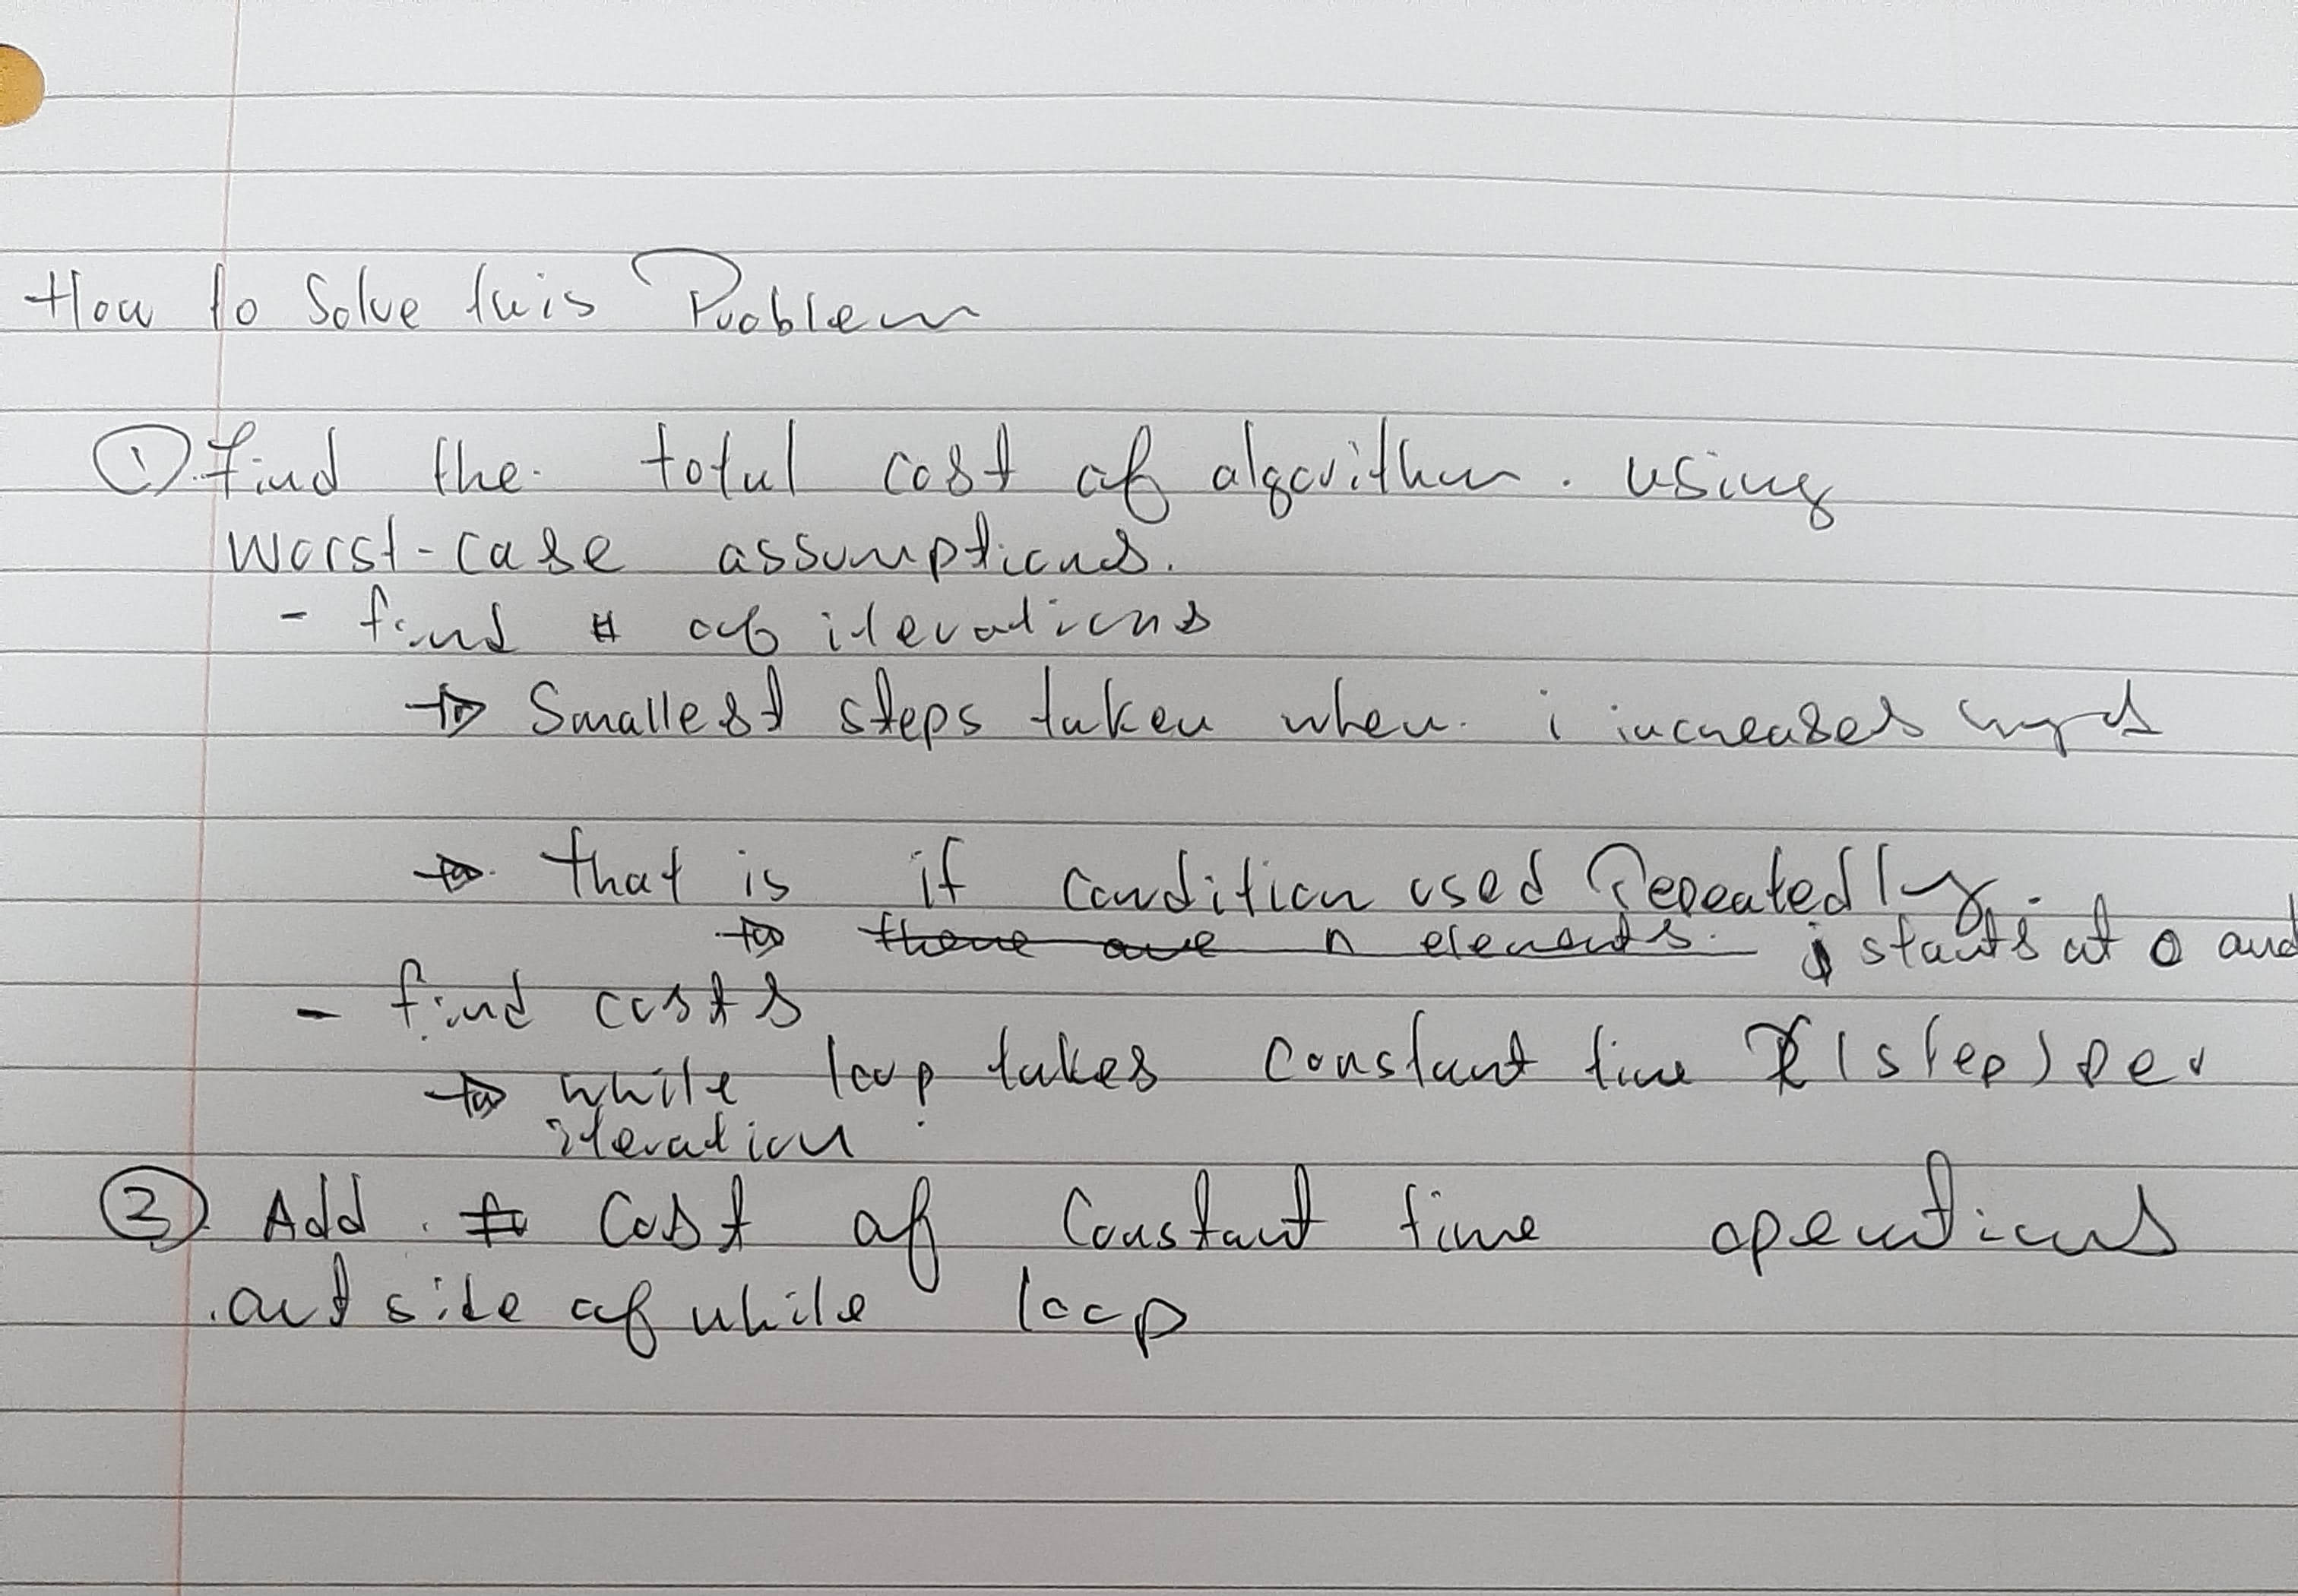
\includegraphics[width=\linewidth]{images/problem_set_4_comments_1.jpg}
        \end{center}

        \item Noticed professor has solution that is a lot different
        than what I thought... Is there concepts I misunderstood?
    \end{itemize}


\end{enumerate}

\section*{Question 4}
\begin{enumerate}[a.]
    \item

    \textbf{Statement:} $\forall n \in \mathbb{Z}^{+},\:\forall k \in \mathbb{N},
    \:\frac{n}{2^k} - \frac{2^k - 1}{2^k} \leq x_k \leq \frac{n}{2^k}$

    \begin{proof}
        We will prove by induction on $k$.

        \bigskip

        \underline{\textbf{Base Case ($k = 0$):}}

        \bigskip

        Let $k = 0$ and $n \in \mathbb{Z}^{+}$.

        \bigskip

        We need to show $n \leq x_0 \leq n$, or $x_0 = n$.

        \bigskip

        It follows from the code that at $0^{th}$ iteration, the value of $x$
        is $n$.

        \bigskip

        \underline{\textbf{Inductive Case ($k \in \mathbb{N}$):}}

        \bigskip

        Let $k \in \mathbb{N}$, and assume the statement is true at $k$.

        \bigskip

        We will to prove $\frac{n}{2^{k+1}} - \frac{2^{k+1}-1}{2^{k+1}} \leq
        x_{k+1} \leq \frac{n}{2^{k+1}}$ in two parts, by showing $\frac{n}{2^{k+1}} -
        \frac{2^{k+1}-1}{2^{k+1}} \leq x_{k+1}$ and $x_{k+1} \leq \frac{n}{2^{k+1}}$.

        \bigskip

        \textbf{Part 1 (Showing $\frac{n}{2^{k+1}} - \frac{2^{k+1}-1}{2^{k+1}} \leq x_{k+1}$):}

        \bigskip

        Starting from $x_{k+1}$, the code tells us

        \setcounter{equation}{0}
        \begin{align}
            x_{k+1} = \left\lfloor \frac{x_k}{2} \right\rfloor
        \end{align}

        \bigskip

        Then, by the hint ($\forall x \in \mathbb{Z}$,
        $\frac{x-1}{2} \leq \left\lfloor \frac{x}{2} \right\rfloor \leq \frac{x}{2}$),
        we can write

        \begin{align}
            x_{k+1} = \left\lfloor \frac{x_k}{2} \right\rfloor &\geq \frac{x_k - 1}{2}\\
            &= \frac{1}{2} \cdot (x_k - 1)
        \end{align}

        \bigskip

        Then, by inductive hypothesis,

        \begin{align}
            x_{k+1} &\geq \frac{1}{2} \cdot \left( \frac{n}{2^k} - \frac{2^k - 1}{2^k} - 1 \right)\\
            &= \frac{n}{2^{k+1}} - \frac{2^k-1}{2^{k+1}} - \frac{1}{2}\\
            &= \frac{n}{2^{k+1}} - \left( \frac{2^k - 1}{2^{k+1}} + \frac{2^k}{2^{k+1}} \right)\\
            &= \frac{n}{2^{k+1}} - \left( \frac{2^k + 2^k - 1}{2^{k+1}} \right)
        \end{align}

        \bigskip

        Then, because we know $2^k + 2^k = 2^{k+1}$, we can conclude

        \begin{align}
            x_{k+1} &\geq \frac{n}{2^{k+1}} - \left( \frac{2^{k+1}-1}{2^{k+1}} \right)
        \end{align}

        \textbf{Part 2 (Showing $x_{k+1} \leq \frac{n}{2^{k+1}}$):}

        \bigskip

        Starting from $x_{k+1}$, the code tells us

        \begin{align}
            x_{k+1} &= \left\lfloor \frac{x_k}{2} \right\rfloor
        \end{align}

        \bigskip

        Then, by the hint ($\forall x \in \mathbb{Z}$, $\frac{x-1}{2} \leq
        \left\lfloor \frac{x}{2} \right\rfloor \leq \frac{x}{2}$), we can write

        \begin{align}
            x_{k+1} = \left\lfloor \frac{x_k}{2} \right\rfloor &\leq \frac{x_k}{2}
        \end{align}

        \bigskip

        Then, by the inductive hypothesis, we can conclude

        \begin{align}
            x_{k+1} &\leq \frac{n}{2^k \cdot 2}\\
            &\leq \frac{n}{2^{k+1}}
        \end{align}
    \end{proof}

    \item

    \textbf{Statement:} $\forall n \in \mathbb{Z}^{+},\:\forall k \in \mathbb{N}$,
    (\textbf{convert\_to\_binary($n$)} takes exactly $k$ loop iterations) $\Leftrightarrow 2^{k-1} \leq n \leq 2^k - 1$

    \bigskip

    \begin{proof}
        Let $n \in \mathbb{Z}$, and $k \in \mathbb{N}$.

        \bigskip

        We will prove the statement in two parts (first is proving in $\Rightarrow$
        direction, and the second is proving in $\Leftarrow$ direction).

        \bigskip

        \textbf{Part 1 (Proving in $\Rightarrow$ direction):}

        \bigskip

        Assume the loop in \textbf{convert\_to\_binary(n)} takes $k$ iterations.

        \bigskip

        We need to prove $2^{k-1} \leq n \leq 2^k - 1$.

        \bigskip

        First, we need to show $2^{k-1} \leq n$.

        \bigskip

        The code tells us at $k^{th}$ iteration $x_k = \left\lfloor
        \frac{x_{k-1}}{2} \right\rfloor$ and $x_k = 0$.

        \bigskip

        Since the assumption tells us $k$ iterations must occur in the loop,
        using these facts, we can conclude $x_{k-1}$ is non-zero.

        \bigskip

        Then, because we know $0 < x_{k-1} = \left\lfloor \frac{x_{k-2}}{2} \right\rfloor \in \mathbb{N}$ and
        $0 = x_0 = \left\lfloor \frac{x_{k-1}}{2} \right\rfloor$, we can conclude $x_{k-1} = 1$.

        \bigskip

        Then, using this fact, with the inequality $\frac{n}{2^k} - \frac{2^k - 1}{2^k} \leq x_k \leq \frac{n}{2^k}$
        from question 4.a, we can conclude

        \bigskip

        \setcounter{equation}{0}
        \begin{align}
            1 = x_{k-1} &\leq \frac{n}{2^{k-1}}\\
            2^{k-1} &\leq n
        \end{align}

        \bigskip

        Now, we need to show $n \leq 2^k - 1$.

        \bigskip

        The code tells us that $x_0 = n$, $x_k = 0$, and from question 4.a,
        $\frac{n}{2^k} - \frac{2^k - 1}{2^k} \leq x_k \leq \frac{n}{2^k}$.

        \bigskip

        Then, using these facts, we can conclude

        \begin{align}
            n - \left( \frac{n}{2^k} - \frac{2^k - 1}{2^k} \right) &\geq x_0 - x_k = n\\
            \frac{2^k \cdot n}{2^k} - \frac{n}{2^k} + \frac{2^k -1}{2^k} &\geq n\\
            \frac{n \cdot (n^k - 1)}{2^k} + \frac{2^k -1}{2^k} &\geq n\\
            \frac{2^k -1}{2^k} &\geq n + \frac{n \cdot (2^k - 1)}{2^k}\\
            \frac{2^k -1}{2^k} &\geq n \cdot \left(\frac{2^k - 2^k + 1}{2^k} \right)\\
            2^k - 1 &\geq n
        \end{align}

        \bigskip

        Since $2^{k-1} \leq n$ and $n \leq 2^k-1$ are true, we can conclude
        $2^{k-1} \leq n \leq 2^k-1$ is true.

        \bigskip

        \textbf{Part 2 (Proving in $\Leftarrow$ direction):}

        \bigskip

        Assume $2^{k-1} \leq n \leq 2^k - 1$.

        \bigskip

        We need to prove that given $n$, the loop in \textbf{convert\_to\_binary(n)}
        takes $k$ iterations.

        \bigskip

        First, we need to show that with the lower bound of $n$, the loop in
        \textbf{convert\_to\_binary(n)} does exactly $k$ iterations.

        \bigskip

        The result of problem 4.a tells us

        \begin{align}
            \forall n \in \mathbb{Z}^{+},\:\forall k \in \mathbb{N},\:\frac{n}{2^k} - \frac{2^k - 1}{2^k} \leq x_k \leq \frac{n}{2^k}
        \end{align}


        Using this fact, we can calculate that the value of $x$ at $k-1^{th}$ iteration is

        \bigskip

        \begin{align}
            \frac{2^{k-1}}{2^{k-1}} - \frac{2^{k-1} - 1}{2^{k-1}} &\leq x_{k-1} \leq \frac{2^{k-1}}{2^{k-1}}\\
            \frac{1}{2^{k-1}} &\leq x_{k-1} \leq 1
        \end{align}

        \bigskip

        Since $\frac{1}{2^{k-1}} > 0$, and $x_{k-1} \in \mathbb{N}$ (from the code),
        we can conclude $x_{k-1} = 1$.

        \bigskip

        Then, by taking an iteration further, we can conclude

        \begin{align}
            x_k &= \left\lfloor \frac{x_{k-1}}{2} \right\rfloor\\
            &= 0
        \end{align}

        \bigskip

        Because we know loop termination occurs when $x \leq 0$, we can conclude
        the loop with lower bound of $n$ stops at $k^{th}$ iteration.

        \bigskip

        Now, we need to show that with $2^k - 1$ as $n$, \textbf{convert\_to\_binary(n)}
        does exactly $k$ iterations.

        \bigskip

        Using equation 9, we can calculate that the value of
        $x$ at $k^{th}$ iteration is

        \bigskip

        \begin{align}
            \frac{2^k - 1}{2^k} - \frac{2^k - 1}{2^k} &\leq x_k \leq \frac{2^k - 1}{2^k}\\
            0 &\leq x_k \leq \frac{2^k - 1}{2^k}
        \end{align}

        \bigskip

        Since we know $\frac{2^k - 1}{2^k} < 1$, and $x_k \in \mathbb{N}$ (from the code),
        we can conclude $x_k = 0$.

        \bigskip

        Because we know loop termination occurs when $x \leq 0$, we can conclude
        the loop with the upper bound of $n$ stops at $k^{th}$ iteration.

        \bigskip

        So, since the loop stops at $k^{th}$ iterations for both the upper
        and the lower bound of $n$, we can conclude $n$ performs exactly
        $k$ iterations.
    \end{proof}

    \bigskip

    \textbf{Notes:}

    \begin{itemize}
        \item This is a tough problem.
        \item 형모 풀꼬얌!! 형모 궁뎡궁뎡 하고 한걸음띡 발쩐해쬬 대학원 갈꼬얌!!
        \item 오예!!! 형모 해낼꼬다!!
        \item 형모 화이팅!!
        \item After hours of thinking, I found the rough idea: find range of values
        between ($x_1 and x_k$) and add to $2^{k-1}$ (where it's the last digit
        of binary number).

        (i.e 10000 and 11111 are two extreme range of values. Here we are finding
        last 4 0000 and 1111, and then adding to first 1).

        \item another one is using $x_0$ and $x_k$.
    \end{itemize}

    \bigskip

    \begin{mdframed}

        \underline{\textbf{Pseudoproof:}}

        \bigskip

        Let $n \in \mathbb{Z}$, and $k \in \mathbb{N}$.

        \bigskip

        We will prove the statement in two parts (first is proving in $\Rightarrow$
        direction, and the second is proving in $\Leftarrow$ direction).

        \bigskip

        \textbf{Part 1 (Proving in $\Rightarrow$ direction):}

        \bigskip

        Assume \textbf{convert\_to\_binary(n)} takes $k$ step.

        \bigskip

        We need to show $2^{k-1} \leq n \leq 2^k - 1$.

        \bigskip

        \begin{enumerate}[1.]
            \item Show $2^{k-1} \leq n$ is true
            \begin{itemize}
                \item Show that $x_{k-1}$ is greater than 1

                \bigskip

                \begin{mdframed}
                    The code tells us $x_k = \left\lfloor \frac{x_{k-1}}{2} \right\rfloor$
                    and at $k^{th}$ iteration $x_k = 0$.

                    \bigskip

                    Since the assumption tells us $k$ iterations must occur, we
                    can conclude $x_{k-1}$ is non-zero.

                    \bigskip

                    Since we know from the code $x_{k-1} \in \mathbb{N}$, we can conclude
                    $x_0 = 0$ will be true when $x_{k-1} = 1$.

                \end{mdframed}

                \bigskip

                \item Show $n \geq 2^{k-1}$

                \bigskip

                \begin{mdframed}
                    Then, using this fact, with the inequality $\frac{n}{2^k} - \frac{2^k - 1}{2^k} \leq x_k \leq \frac{n}{2^k}$
                    from the result of question 4.a, we can conclude

                    \bigskip

                    \begin{align}
                        1 = x_{k-1} &\leq \frac{n}{2^{k-1}}\\
                        2^{k-1} &\leq n
                    \end{align}
                \end{mdframed}

            \end{itemize}

            \item Show $n \leq 2^k - 1$ is true

            \begin{itemize}
                \item start from the left and move to the right

                \begin{itemize}
                    \item Show that $x_0 = n$, $x_k = 0$ and $\frac{n}{2^k} - \frac{2^k - 1}{2^k} \leq x_k \leq \frac{n}{2^k}$

                    \begin{mdframed}
                    The code tells us that $x_0 = n$, $x_k = 0$, and from the result of question 4.a,
                    we know $\frac{n}{2^k} - \frac{2^k - 1}{2^k} \leq x_k \leq \frac{n}{2^k}$.
                    \end{mdframed}

                    \item Use these facts to calculate that $2^k - 1 \geq n$

                    \begin{mdframed}
                    Then, using these facts, we can conclude

                    \begin{align}
                        n - \left( \frac{n}{2^k} - \frac{2^k - 1}{2^k} \right) &\geq x_0 - x_k = n\\
                        \frac{2^k \cdot n}{2^k} - \frac{n}{2^k} + \frac{2^k -1}{2^k} &\geq n\\
                        \frac{n \cdot (n^k - 1)}{2^k} + \frac{2^k -1}{2^k} &\geq n\\
                        \frac{2^k -1}{2^k} &\geq n + \frac{n \cdot (2^k - 1)}{2^k}\\
                        \frac{2^k -1}{2^k} &\geq n \cdot \left(\frac{2^k - 2^k + 1}{2^k} \right)\\
                        2^k - 1 &\geq n
                    \end{align}
                    \end{mdframed}
                \end{itemize}
            \end{itemize}

            \item Conclusion (combine parts together)

            \begin{mdframed}
            Since $2^{k-1} \leq n$ and $n \leq 2^k-1$ are true, we can conclude
            $2^{k-1} \leq n \leq 2^k-1$ is true.
            \end{mdframed}
        \end{enumerate}

        \bigskip

        \textbf{Part 2 (Proving in $\Leftarrow$ direction):}

        \bigskip

        Assume $2^{k-1} \leq n \leq 2^k - 1$.

        \bigskip

        We need to show \textbf{convert\_to\_binary(n)} takes $k$ step.

        \bigskip

        \begin{enumerate}[1.]
            \item Show that with $2^{k-1}$ as $n$, \textbf{convert\_to\_binary(n)}
            does exactly $k$ iterations.

            \bigskip

            \begin{mdframed}
            For the lower bound of $n$, using the result of problem 4.a $\frac{n}{2^k} - \frac{2^k - 1}{2^k}
            \leq x_k \leq \frac{n}{2^k}$, we can calculate that the value of $x$
            at $k-1^{th}$ iteration is

            \bigskip

            \begin{align}
                \frac{2^{k-1}}{2^{k-1}} - \frac{2^{k-1} - 1}{2^{k-1}} &\leq x_{k-1} \leq \frac{2^{k-1}}{2^{k-1}}\\
                \frac{1}{2^{k-1}} &\leq x_{k-1} \leq 1
            \end{align}

            \bigskip

            Since we know $\frac{1}{2^{k-1}} > 0$, and $x_{k-1} \in \mathbb{N}$ (from the code),
            we can conclude $x_{k-1} = 1$.

            \bigskip

            Then, by taking an iteration further, we can conclude

            \begin{align}
                x_k &= \left\lfloor \frac{x_{k-1}}{2} \right\rfloor\\
                &= 0
            \end{align}

            \bigskip

            Because we know loop termination occurs when $x \leq 0$, we can conclude
            the loop with the lower bound of $n$ stops at $k^{th}$ iteration.

            \end{mdframed}

            \bigskip

            \item Show that with $2^k - 1$ as $n$, \textbf{convert\_to\_binary(n)}
            does exactly $k$ iterations.

            \bigskip

            \begin{mdframed}
            For the upper bound of $n$, using the same result from problem 4.a,
            the value of $x$ at $k^{th}$ iteration is

            \bigskip

            \begin{align}
                \frac{2^k - 1}{2^k} - \frac{2^k - 1}{2^k} &\leq x_k \leq \frac{2^k - 1}{2^k}\\
                0 &\leq x_k \leq \frac{2^k - 1}{2^k}
            \end{align}

            \bigskip

            Since we know $\frac{2^k - 1}{2^k} < 1$, and $x_k \in \mathbb{N}$ (from the code),
            we can conclude $x_k = 0$.

            \bigskip

            Because we know loop termination occurs when $x \leq 0$, we can conclude
            the loop with the upper bound of $n$ stops at $k^{th}$ iteration.

            \end{mdframed}

            \item Conclude $n$ performs $k$ iterations.

            \bigskip

            \begin{mdframed}
            So, since the loop stops at $k^{th}$ iterations for both the upper
            and the lower bound of $n$, we can conclude $n$ performs exactly
            $k$ iterations.
            \end{mdframed}

        \end{enumerate}

    \end{mdframed}

    \item

    Let $n \in \mathbb{Z}^+$, $k \in \mathbb{N}$ and let $S_k$ denote the set
    of all numbers resulting in $k$ many iterations in \textbf{convert\_to\_binary(n)}.

    \bigskip

    We need to evaluate the following expression

    \setcounter{equation}{0}
    \begin{align}
        AVG_{convert\_to\_binary}(n) &= \frac{1}{\lvert \mathcal{I}_n \rvert} \sum\limits_{i \in \mathcal{I}_n} \text{Running time of convert\_to\_binary}
    \end{align}

    \bigskip

    First, we need to show set of $S_k$ over all $k$ are partitions of $\mathcal{I}_n$.
    That is, the union of all of $S_k$ form $\mathcal{I}_n$ and $S_k$ over all $k$ do
    not have any elements in common.

    \bigskip

    The question 4.b tells us

    \begin{align}
        \begin{split}
        \forall n \in \mathbb{Z}^+, \forall k \in \mathbb{N},\: (\textbf{
        convert\_to\_binary(n)}\:\text{takes exactly}\:k\:\text{loop iterations}) \Leftrightarrow
        \\ 2^{k-1} \leq n \leq 2^k -1
        \end{split}
    \end{align}

    Using this fact, we can conclude $S_k$ has highest element with the value of $2^k - 1$,
    and $S_{k+1}$ has element with the lowest value of $2^{k+1-1}=2^k$.

    \bigskip

    Then, we can calculate that

    \begin{align}
        2^k - (2^k - 1) = 1
    \end{align}

    \bigskip

    Then, because we know the distance between the two sets have value greater than 0, we can
    conclude the two sets are non-overlapping, and do not have elements in common.

    \bigskip

    Now, we know $S_k$ is the result of grouping elements in $\mathcal{I}_n$.

    \bigskip

    It follows from this fact that it's union form $\mathcal{I}_n$.

    \bigskip

    Second, we need to evaluate the number of input elements $\lvert \mathcal{I}_n \rvert$.

    \bigskip

    Because we know $\mathcal{I}_n$ has all integer elements from $1$ to $2^n - 1$,
    we can conclude

    \begin{align}
        \lvert \mathcal{I}_n \rvert &= 2^n - 1 - 1 + 1\\
        &= 2^n - 1
    \end{align}

    \bigskip

    Third, we need to determine the smallest and the largest value of $k$
    of $S_k$ in $\mathcal{I}_n$

    \bigskip

    We will do so in parts.

    \bigskip

    \textbf{Part 1 (Finding the smallest value of $k$):}

    \bigskip

    We need to find the smallest value of $k$.

    \bigskip

    The code tells us the value of $k$ rises as $n$ increases.

    \bigskip

    Because we know 1 is the smallest value in $\mathcal{I}_n$, we can conclude
    $1$ is the value that will result in smallest value of $k$.

    \bigskip

    Now, the question 4.b tells us

    \begin{align}
        \begin{split}
        \forall n \in \mathbb{Z}^+, \forall k \in \mathbb{N},\: (\textbf{
        convert\_to\_binary(n)}\:\text{takes exactly}\:k\:\text{loop iterations}) \Leftrightarrow
        \\ 2^{k-1} \leq n \leq 2^k -1
        \end{split}
    \end{align}

    Because we know $1 = 2^{1 - 1}$, by using the fact, we can conclude $k = 1$.

    \bigskip

    \textbf{Part 2 (Finding the largest value of $k$):}

    \bigskip

    We need to find the largest value of $k$.

    \bigskip

    The code tells us the value of $k$ rises as $n$ increases.

    \bigskip

    Since the highest value in $\mathcal{I}_n$ is $2^n - 1$, we can conclude
    $2^n - 1$ is the value that will result in highest value of $k$.

    \bigskip

    Now, The question 4.b tells us

    \begin{align}
        \begin{split}
        \forall n \in \mathbb{Z}^+, \forall k \in \mathbb{N},\: (\textbf{
        convert\_to\_binary(n)}\:\text{takes exactly}\:k\:\text{loop iterations}) \Leftrightarrow
        \\ 2^{k-1} \leq n \leq 2^k -1
        \end{split}
    \end{align}

    \bigskip

    Using this fact, we can conclude $k$ has the highest value of $n$.

    \bigskip

    Fourth, we need to show $\lvert S_k \rvert = 2^{k-1}$ for $k = 1 \dots n$.

    \bigskip

    We will do so using proof by cases.

    \bigskip

    \textbf{Case 1 ($k = 1 \dots n-1$):}

    \bigskip

    In this case, we need to show $\lvert S_k \rvert = 2^{k-1}$
    for $k = 1 \dots n-1$.

    \bigskip

    The question 4.b tells us

    \begin{align}
        \begin{split}
        \forall n \in \mathbb{Z}^+, \forall k \in \mathbb{N},\: (\textbf{
        convert\_to\_binary(n)}\:\text{takes exactly}\:k\:\text{loop iterations}) \Leftrightarrow
        \\ 2^{k-1} \leq n \leq 2^k -1
        \end{split}
    \end{align}

    \bigskip

    Because we know no elements are missing in $S_k$,
    by using this fact, we can calculate that

    \begin{align}
        \lvert S_k \rvert &= 2^k -1 - 2^{k-1} + 1\\
        &= 2^k - 2^{k-1}\\
        &= 2^{k-1}
    \end{align}

    \bigskip

    \textbf{Case 2 ($k = n$):}

    \bigskip

    In this case, we need to show $\lvert S_k \rvert = 2^{k-1}$
    for $k = n$.

    \bigskip

    The question 4.b tells us

    \begin{align}
        \begin{split}
        \forall n \in \mathbb{Z}^+, \forall k \in \mathbb{N},\: (\textbf{
        convert\_to\_binary(n)}\:\text{takes exactly}\:k\:\text{loop iterations}) \Leftrightarrow
        \\ 2^{k-1} \leq n \leq 2^k -1
        \end{split}
    \end{align}

    \bigskip

    Using this fact, we know the value of last element in $S_{n-1}$
    is $2^{n-1} - 1$.

    \bigskip

    Because we know elements in $\mathcal{I}_n$ increases by 1,
    we can conclude the value of first element in $S_n$ is

    \begin{align}
        2^{n-1} - 1 + 1 = 2^{n-1}
    \end{align}

    \bigskip

    Now, because we know the first element in $S_n$ is $2^{n-1}$
    and the last element in $S_n$ is $2^n -1$, using
    these fact, we can conclude

    \begin{align}
        \lvert S_k \rvert &= 2^{n-1} - (2^{n-1} - 1) + 1\\
        &= 2^n - 2^{n-1}\\
        &= 2^{n-1}\\
        &= 2^{k-1}
    \end{align}

    \bigskip

    Fifth, we need to evaluate the running time of \textbf{convert\_to\_binary(n)}
    for all elements in $S_k$.

    \bigskip

    The header tells us that elements in $S_k$ result in loop with $k$ iterations, and
    the code tells us each loop takes constant time (1 step).

    \bigskip

    Using these facts, we can calculate the loop has total time of

    \begin{align}
        k \cdot 1 = k
    \end{align}

    steps.

    \bigskip

    Since we are ignoring the time of constant operations outside of the loop,
    we can conclude \textbf{convert\_to\_binary(n)} has running time of $k$ steps.

    \bigskip

    Sixth, we need to re-express the average-case running time as sum over $S_k$.

    \bigskip

    Because we know the sets $S_k$ over $k = 1 \dots n$ are partitions of
    $\mathcal{I}_n$, we can conclude $\sum\limits_{i \in \mathcal{I}_n}$
    is the same as $\sum\limits_{k = 1}^n \sum\limits_{i \in S_k}$.

    \bigskip

    Using this fact, we can write

    \begin{align}
        AVG_{\text{convert\_to\_binary}}(n) &= \frac{1}{\lvert \mathcal{I}_n \rvert} \cdot \sum\limits_{k = 1}^n \sum\limits_{i \in S_k} \text{Runtime of convert\_to\_binary}
    \end{align}

    \bigskip

    Then, because we know all values in $\lvert S_k \rvert$ has the same
    running time, we can write

    \begin{align}
        AVG_{\text{convert\_to\_binary}}(n) &= \frac{1}{\lvert \mathcal{I}_n \rvert} \cdot \sum\limits_{k = 1}^n \lvert S_k \rvert \cdot \text{Runtime of convert\_to\_binary}
    \end{align}

    \bigskip

    Then, since we know $\lvert \mathcal{I}_n \rvert = 2^n - 1$, and
    $\lvert S_k \rvert = 2^{k-1}$, we can write

    \begin{align}
        AVG_{\text{convert\_to\_binary}}(n) &= \frac{1}{2^n - 1} \cdot \sum\limits_{k = 1}^n 2^{k-1} \cdot \text{Runtime of convert\_to\_binary}
    \end{align}

    \bigskip

    Then, because we know all elements in $S_k$ has runtime of $k$,
    we can conclude

    \begin{align}
        AVG_{\text{convert\_to\_binary}}(n) &= \frac{1}{2^n - 1} \cdot \sum\limits_{k = 1}^n 2^{k-1} \cdot k
    \end{align}

    \bigskip

    Finally, we need to evaluate the average-case running time of\\
    \textbf{convert\_to\_binary(n)}.

    \bigskip

    The hint tells us

    \begin{align}
        \forall m \in \mathbb{N},\:\forall r \in \mathbb{R},\:\sum\limits_{i=1}^m ir^{i-1} = \frac{1 - r^{m+1}}{(1-r)^2} - \frac{(m+1)r^m}{1-r}\:\text{where}\:r \neq 1
    \end{align}

    \bigskip

    Using the hint, we can conclude

    \begin{align}
        AVG_{\text{convert\_to\_binary}}(n) &= \frac{1}{2^n - 1} \cdot \sum\limits_{k = 1}^n 2^{k-1} \cdot k\\
        &= \frac{1}{2^n - 1} \cdot \left[ \frac{1 - 2^{n+1}}{(1-2)^2} - \frac{(n+1)2^n}{1-2} \right]\\
        &= \frac{1}{2^n - 1} \cdot \left[ 1 - 2^{n+1} + (n+1)2^n \right]\\
        &= \frac{1}{2^n - 1} \cdot \left[ 1 - 2 \cdot 2^n + (n+1)2^n \right]\\
        &= \frac{1}{2^n - 1} \cdot \left[ 1 - 2 \cdot 2^n + (n+1)2^n \right]\\
        &= \frac{1}{2^n - 1} \cdot \left[ 1 + 2^n(n+1 - 2) \right]\\
        &= \frac{1}{2^n - 1} \cdot \left[ 1 + 2^n(n-1) \right]
    \end{align}

    \bigskip

    \begin{mdframed}

    \underline{\textbf{Rough Work:}}

    \bigskip

    \begin{enumerate}[1.]

        \item Show set of $S_k$ over all $k$ are partitions of $\mathcal{I}_n$.

        \begin{mdframed}
            First, we need to show set of $S_k$ over all $k$ are partitions of $\mathcal{I}_n$.
            That is, the union of all of $S_k$ form $\mathcal{I}_n$ and $S_k$ over all $k$ do
            not have any elements in common.

            \bigskip

            The question 4.b tells us

            \begin{align}
                \begin{split}
                \forall n \in \mathbb{Z}^+, \forall k \in \mathbb{N},\: (\textbf{
                convert\_to\_binary(n)}\:\text{takes exactly}\:k\:\text{loop iterations}) \Leftrightarrow
                \\ 2^{k-1} \leq n \leq 2^k -1
                \end{split}
            \end{align}

            Using this fact, we can conclude $S_k$ has highest element with the value of $2^k - 1$,
            and $S_{k+1}$ has element with the lowest value of $2^{k+1-1}=2^k$.

            \bigskip

            Then, we can calculate that

            \begin{align}
                2^k - (2^k - 1) = 1
            \end{align}

            \bigskip

            Then, because we know the distance between the two sets have value greater than 0, we can
            conclude the two sets are non-overlapping, and do not have elements in common.

            \bigskip

            Now, we know $S_k$ is the result of grouping elements in $\mathcal{I}_n$.

            \bigskip

            It follows from this fact that it's union form $\mathcal{I}_n$.
        \end{mdframed}

        \item Find the number of input elements $\lvert \mathcal{I}_n \rvert$.

        \begin{mdframed}
        Second, we need to evaluate the number of input elements $\lvert \mathcal{I}_n \rvert$.

        \bigskip

        Because we know $\mathcal{I}_n$ has all integer elements from $1$ to $2^n - 1$,
        we can conclude

        \begin{align}
            \lvert \mathcal{I}_n \rvert &= 2^n - 1 - 1 + 1\\
            &= 2^n - 1
        \end{align}
        \end{mdframed}

        \item Find the first and last value of $k$ of $S_k$ in $\mathcal{I}_n$.

        \begin{mdframed}
        Third, we need to determine the smallest and the largest value of $k$
        of $S_k$ in $\mathcal{I}_n$

        \bigskip

        We will do so in parts.

        \bigskip

        \textbf{Part 1 (Finding the smallest value of $k$):}

        \bigskip

        We need to find the smallest value of $k$.

        \bigskip

        The code tells us the value of $k$ rises as $n$ increases.

        \bigskip

        Because we know 1 is the smallest value in $\mathcal{I}_n$, we can conclude
        $1$ is the value that will result in smallest value of $k$.

        \bigskip

        Now, the question 4.b tells us

        \begin{align}
            \begin{split}
            \forall n \in \mathbb{Z}^+, \forall k \in \mathbb{N},\: (\textbf{
            convert\_to\_binary(n)}\:\text{takes exactly}\:k\:\text{loop iterations}) \Leftrightarrow
            \\ 2^{k-1} \leq n \leq 2^k -1
            \end{split}
        \end{align}

        Because we know $1 = 2^{1 - 1}$, by using the fact, we can conclude $k = 1$.

        \bigskip

        \textbf{Part 2 (Finding the largest value of $k$):}

        \bigskip

        We need to find the largest value of $k$.

        \bigskip

        The code tells us the value of $k$ rises as $n$ increases.

        \bigskip

        Since the highest value in $\mathcal{I}_n$ is $2^n - 1$, we can conclude
        $2^n - 1$ is the value that will result in highest value of $k$.

        \bigskip

        Now, The question 4.b tells us

        \begin{align}
            \begin{split}
            \forall n \in \mathbb{Z}^+, \forall k \in \mathbb{N},\: (\textbf{
            convert\_to\_binary(n)}\:\text{takes exactly}\:k\:\text{loop iterations}) \Leftrightarrow
            \\ 2^{k-1} \leq n \leq 2^k -1
            \end{split}
        \end{align}

        \bigskip

        Using this fact, we can conclude $k$ has the highest value of $n$.
        \end{mdframed}

        \item Show the number of $\lvert S_k \rvert = 2^{k-1}$.

        \bigskip

        Fourth, we need to show $\lvert S_k \rvert = 2^{k-1}$ for $k = 1 \dots n$.

        \bigskip

        We will do so using proof by cases.

        \bigskip

        \begin{enumerate}[1.]
            \item Case 1 ($k = 1 \dots n-1$):

            \begin{mdframed}
            In this case, we need to show $\lvert S_k \rvert = 2^{k-1}$
            for $k = 1 \dots n-1$.

            \bigskip

            The question 4.b tells us

            \begin{align}
                \begin{split}
                \forall n \in \mathbb{Z}^+, \forall k \in \mathbb{N},\: (\textbf{
                convert\_to\_binary(n)}\:\text{takes exactly}\:k\:\text{loop iterations}) \Leftrightarrow
                \\ 2^{k-1} \leq n \leq 2^k -1
                \end{split}
            \end{align}

            \bigskip

            Because we know no elements are missing in $S_k$,
            by using this fact, we can calculate that

            \begin{align}
                \lvert S_k \rvert &= 2^k -1 - 2^{k-1} + 1\\
                &= 2^k - 2^{k-1}\\
                &= 2^{k-1}
            \end{align}
            \end{mdframed}

            \item Case 2 ($k = n$):

            \begin{mdframed}
            In this case, we need to show $\lvert S_k \rvert = 2^{k-1}$
            for $k = n$.

            \bigskip

            The question 4.b tells us

            \begin{align}
                \begin{split}
                \forall n \in \mathbb{Z}^+, \forall k \in \mathbb{N},\: (\textbf{
                convert\_to\_binary(n)}\:\text{takes exactly}\:k\:\text{loop iterations}) \Leftrightarrow
                \\ 2^{k-1} \leq n \leq 2^k -1
                \end{split}
            \end{align}

            \bigskip

            Using this fact, we know the value of last element in $S_{n-1}$
            is $2^{n-1} - 1$.

            \bigskip

            Because we know elements in $\mathcal{I}_n$ increases by 1,
            we can conclude the value of first element in $S_n$ is

            \begin{align}
                2^{n-1} - 1 + 1 = 2^{n-1}
            \end{align}

            \bigskip

            Now, because we know the first element in $S_n$ is $2^{n-1}$
            and the last element in $S_n$ is $2^n -1$, using
            these fact, we can conclude

            \begin{align}
                \lvert S_k \rvert &= 2^{n-1} - (2^{n-1} - 1) + 1\\
                &= 2^n - 2^{n-1}\\
                &= 2^{n-1}\\
                &= 2^{k-1}
            \end{align}
            \end{mdframed}
        \end{enumerate}

        \bigskip

        \begin{mdframed}
            Fourth, we need to show $\lvert S_k \rvert = 2^{k-1}$ for $k = 1 \dots n$.

            \bigskip

            We will do so using proof by cases.

            \bigskip

            \textbf{Case 1 ($k = 1 \dots n-1$):}

            \bigskip

            In this case, we need to show $\lvert S_k \rvert = 2^{k-1}$
            for $k = 1 \dots n-1$.

            \bigskip

            The question 4.b tells us

            \begin{align}
                \begin{split}
                \forall n \in \mathbb{Z}^+, \forall k \in \mathbb{N},\: (\textbf{
                convert\_to\_binary(n)}\:\text{takes exactly}\:k\:\text{loop iterations}) \Leftrightarrow
                \\ 2^{k-1} \leq n \leq 2^k -1
                \end{split}
            \end{align}

            \bigskip

            Because we know no elements are missing in $S_k$,
            by using this fact, we can calculate that

            \begin{align}
                \lvert S_k \rvert &= 2^k -1 - 2^{k-1} + 1\\
                &= 2^k - 2^{k-1}\\
                &= 2^{k-1}
            \end{align}

            \bigskip

            \textbf{Case 2 ($k = n$):}

            \bigskip

            In this case, we need to show $\lvert S_k \rvert = 2^{k-1}$
            for $k = n$.

            \bigskip

            The question 4.b tells us

            \begin{align}
                \begin{split}
                \forall n \in \mathbb{Z}^+, \forall k \in \mathbb{N},\: (\textbf{
                convert\_to\_binary(n)}\:\text{takes exactly}\:k\:\text{loop iterations}) \Leftrightarrow
                \\ 2^{k-1} \leq n \leq 2^k -1
                \end{split}
            \end{align}

            \bigskip

            Using this fact, we know the value of last element in $S_{n-1}$
            is $2^{n-1} - 1$.

            \bigskip

            Because we know elements in $\mathcal{I}_n$ increases by 1,
            we can conclude the value of first element in $S_n$ is

            \begin{align}
                2^{n-1} - 1 + 1 = 2^{n-1}
            \end{align}

            \bigskip

            Now, because we know the first element in $S_n$ is $2^{n-1}$
            and the last element in $S_n$ is $2^n -1$, using
            these fact, we can conclude

            \begin{align}
                \lvert S_k \rvert &= 2^{n-1} - (2^{n-1} - 1) + 1\\
                &= 2^n - 2^{n-1}\\
                &= 2^{n-1}\\
                &= 2^{k-1}
            \end{align}

        \end{mdframed}

        \item Evaluate the running time of \textbf{convert\_to\_binary(n)} for all
        elements in $S_k$.

        \bigskip

        Fifth, we need to evaluate the running time of \textbf{convert\_to\_binary(n)}
        for all elements in $S_k$.

        \bigskip

        \begin{itemize}
            \item State that elements in $S_k$ result in loop with $k$ iterations, and
            that each loop in \textbf{convert\_to\_binary(n)} takes
            a constant time (1 step)

            \begin{mdframed}
            The header tells us that elements in $S_k$ result in loop with $k$ iterations, and
            the code tells us each loop takes a constant time (1 step).
            \end{mdframed}

            \item Show the loop has total time of $k$ steps

            \begin{mdframed}
            Using these facts, we can calculate the loop has total time of

            \begin{align}
                k \cdot 1 = k
            \end{align}

            steps.
            \end{mdframed}

            \item Show \textbf{convert\_to\_binary(n)} has running time of $k$ steps.

            \begin{mdframed}
            Since we are ignoring the time of constant operations outside of the loop,
            we can conclude \textbf{convert\_to\_binary(n)} has running time of $k$ steps.
            \end{mdframed}
        \end{itemize}

        \begin{mdframed}

        Fifth, we need to evaluate the running time of \textbf{convert\_to\_binary(n)}
        for all elements in $S_k$.

        \bigskip

        The header tells us that elements in $S_k$ result in loop with $k$ iterations, and
        the code tells us each loop takes constant time (1 step).

        \bigskip

        Using these facts, we can calculate the loop has total time of

        \begin{align}
            k \cdot 1 = k
        \end{align}

        steps.

        \bigskip

        Since we are ignoring the time of constant operations outside of the loop,
        we can conclude \textbf{convert\_to\_binary(n)} has running time of $k$ steps.

        \end{mdframed}

        \item Re-express the average-case running time as sum over $S_k$.

        \bigskip

        Sixth, we need to re-express the average-case running time as sum over $S_k$.

        \bigskip

        \begin{mdframed}

            Sixth, we need to re-express the average-case running time as sum over $S_k$.

            \bigskip

            Because we know the sets $S_k$ over $k = 1 \dots n$ are partitions of
            $\mathcal{I}_n$, we can conclude $\sum\limits_{i \in \mathcal{I}_n}$
            is the same as $\sum\limits_{k = 1}^n \sum\limits_{i \in S_k}$.

            \bigskip

            Using this fact, we can write

            \begin{align}
                AVG_{\text{convert\_to\_binary}}(n) &= \frac{1}{\lvert \mathcal{I}_n \rvert} \cdot \sum\limits_{k = 1}^n \sum\limits_{i \in S_k} \text{Runtime of convert\_to\_binary}
            \end{align}

            \bigskip

            Then, because we know all values in $\lvert S_k \rvert$ has the same
            running time, we can write

            \begin{align}
                AVG_{\text{convert\_to\_binary}}(n) &= \frac{1}{\lvert \mathcal{I}_n \rvert} \cdot \sum\limits_{k = 1}^n \lvert S_k \rvert \cdot \text{Runtime of convert\_to\_binary}
            \end{align}

            \bigskip

            Then, since we know $\lvert \mathcal{I}_n \rvert = 2^n - 1$, and
            $\lvert S_k \rvert = 2^{k-1}$, we can write

            \begin{align}
                AVG_{\text{convert\_to\_binary}}(n) &= \frac{1}{2^n - 1} \cdot \sum\limits_{k = 1}^n 2^{k-1} \cdot \text{Runtime of convert\_to\_binary}
            \end{align}

            \bigskip

            Then, because we know all elements in $S_k$ has runtime of $k$,
            we can conclude

            \begin{align}
                AVG_{\text{convert\_to\_binary}}(n) &= \frac{1}{2^n - 1} \cdot \sum\limits_{k = 1}^n 2^{k-1} \cdot k
            \end{align}

        \end{mdframed}

        \item Evaluate the average case running time.

        \bigskip

        Finally, we need to evaluate the average-case running time of
        \textbf{convert\_to\_binary(n)}.

        \bigskip

        \begin{itemize}
            \item State the hint, and the average-case running time

            \begin{mdframed}

            The hint tells us

            \begin{align}
                \forall m \in \mathbb{N},\:\forall r \in \mathbb{R},\:\sum\limits_{i=1}^m ir^{i-1} = \frac{1 - r^{m+1}}{(1-r)^2} - \frac{(m+1)r^m}{1-r}\:\text{where}\:r \neq 1
            \end{align}

            \end{mdframed}

            \item Evaluate the expression using the hint

            \begin{mdframed}

            Using the hint, we can conclude

            \begin{align}
                AVG_{\text{convert\_to\_binary}}(n) &= \frac{1}{2^n - 1} \cdot \sum\limits_{k = 1}^n 2^{k-1} \cdot k\\
                &= \frac{1}{2^n - 1} \cdot \left[ \frac{1 - 2^{n+1}}{(1-2)^2} - \frac{(n+1)2^n}{1-2} \right]\\
                &= \frac{1}{2^n - 1} \cdot \left[ 1 - 2^{n+1} + (n+1)2^n \right]\\
                &= \frac{1}{2^n - 1} \cdot \left[ 1 - 2 \cdot 2^n + (n+1)2^n \right]\\
                &= \frac{1}{2^n - 1} \cdot \left[ 1 - 2 \cdot 2^n + (n+1)2^n \right]\\
                &= \frac{1}{2^n - 1} \cdot \left[ 1 + 2^n(n+1 - 2) \right]\\
                &= \frac{1}{2^n - 1} \cdot \left[ 1 + 2^n(n-1) \right]
            \end{align}

            \end{mdframed}
        \end{itemize}

        \begin{mdframed}

            Finally, we need to evaluate the average-case running time of\\
            \textbf{convert\_to\_binary(n)}.

            \bigskip

            The hint tells us

            \begin{align}
                \forall m \in \mathbb{N},\:\forall r \in \mathbb{R},\:\sum\limits_{i=1}^m ir^{i-1} = \frac{1 - r^{m+1}}{(1-r)^2} - \frac{(m+1)r^m}{1-r}\:\text{where}\:r \neq 1
            \end{align}

            \bigskip

            Using the hint, we can conclude

            \begin{align}
                AVG_{\text{convert\_to\_binary}}(n) &= \frac{1}{2^n - 1} \cdot \sum\limits_{k = 1}^n 2^{k-1} \cdot k\\
                &= \frac{1}{2^n - 1} \cdot \left[ \frac{1 - 2^{n+1}}{(1-2)^2} - \frac{(n+1)2^n}{1-2} \right]\\
                &= \frac{1}{2^n - 1} \cdot \left[ 1 - 2^{n+1} + (n+1)2^n \right]\\
                &= \frac{1}{2^n - 1} \cdot \left[ 1 - 2 \cdot 2^n + (n+1)2^n \right]\\
                &= \frac{1}{2^n - 1} \cdot \left[ 1 - 2 \cdot 2^n + (n+1)2^n \right]\\
                &= \frac{1}{2^n - 1} \cdot \left[ 1 + 2^n(n+1 - 2) \right]\\
                &= \frac{1}{2^n - 1} \cdot \left[ 1 + 2^n(n-1) \right]
            \end{align}
        \end{mdframed}
    \end{enumerate}

    \end{mdframed}

    \bigskip

    \textbf{Notes:}

    \begin{itemize}
        \item 따뜻한 내 여보 향해 한걸음 더!!!!
        \item 울지마 형모야.
        \item 주저 앉지마 형모야.
        \item 할 수 있어.
    \end{itemize}

\end{enumerate}

\end{document}